% ****** Start of file aipsamp.tex ******
%
%   This file is part of the AIP files in the AIP distribution for REVTeX 4.
%   Version 4.1 of REVTeX, October 2009
%
%   Copyright (c) 2009 American Institute of Physics.
%
%   See the AIP README file for restrictions and more information.
%
% TeX'ing this file requires that you have AMS-LaTeX 2.0 installed
% as well as the rest of the prerequisites for REVTeX 4.1
%
% It also requires running BibTeX. The commands are as follows:
%
%  1)  latex  aipsamp
%  2)  bibtex aipsamp
%  3)  latex  aipsamp
%  4)  latex  aipsamp
%
% Use this file as a source of example code for your aip document.
% Use the file aiptemplate.tex as a template for your document.
\documentclass[%
 aip,
%jmp,%
%bmf,%
%sd,%
rsi,%
 amsmath,amssymb,
%preprint,%
reprint,%
%author-year,%
%author-numerical,%
]{revtex4-1}

\usepackage{graphicx}% Include figure files
\usepackage{dcolumn}% Align table columns on decimal point
\usepackage{bm}% bold math
%\usepackage[mathlines]{lineno}% Enable numbering of text and display math
%\linenumbers\relax % Commence numbering lines

\usepackage[T1]{fontenc}
\usepackage[utf8]{inputenc}
\usepackage[polutonikogreek,english]{babel}
\usepackage{hyperref}
\hypersetup{colorlinks=true,allcolors=blue}
\usepackage[all]{hypcap}

\newcommand{\micron}{\textgreek{μ}m}
\newcommand{\microsec}{\textgreek{μ}s}
\newcommand{{\usalex}}{\textgreek{μ}sALEX}

\begin{document}

\preprint{AIP/123-QED}

\title[48-spot draft]{48-spot single-molecule FRET setup with periodic acceptor excitation}

\author{Antonino Ingargiola}%
 \email{ingargiola.antonino@gmail.com}
\author{Maya Segal}
\affiliation{
Dept. Chemistry and Biochemistry, University of California Los Angeles, USA}
\author{Angelo Gulinatti}
\author{Ivan Rech}
\author{Massimo Ghioni}
\affiliation{%
DEIB, Politecnico di Milano, Italy
}%
\author{Shimon Weiss}%
\author{Xavier Michalet}%
 \email{michalet@chem.ucla.edu}
\affiliation{
Dept. Chemistry and Biochemistry, University of California Los Angeles, USA}


\date{\today}% It is always \today, today,
             %  but any date may be explicitly specified

\begin{abstract}
Single-molecule FRET (smFRET) allows measuring distances between a donor (D) and
an acceptor (A) fluorophore on the 3-10~nm scale range.
Solution-based smFRET  allows measuring binding-unbinding
or conformational changes of dye-labeled biomolecules without ensemble averaging
and free from perturbation from surfaces binding. When employing dual (or multi)
laser excitation, the technique allows resolving the number of fluorescent
labels on each molecule, greatly enhancing the ability to study heterogeneous
samples.
A major drawback of solution-based smFRET technique is the low throughput,
which renders repetitive measurements expensive and hinder the ability
to study kinetic phenomena in realtime.

Here we demonstrate an high-throughput single-molecule FRET system which
multiplexes the acquisition by using 48 excitation spots and
48-pixels SPAD array detectors. The systems employs two excitation lasers
allowing the separation of doubly- and singly-labeled species.
The performances of the systems are demonstrated on a set of dual-labeled
double-stranded DNA oligos with different D and A dye separations.
We show that the acquisition time for accurate sub-population identification
is reduced from several minutes to seconds, opening the way
to high-throughput screening applications as well as
to realtime kinetics studies of enzymatic reactions such
as DNA transcription by RNA polymerase.
\end{abstract}

\keywords{Single-molecule FRET, high-throughput, SPAD array}
%Use showkeys class option if keyword display desired
\maketitle

\section{Introduction} \label{sec:intro}

Single-molecule FRET (smFRET) studies of freely-diffusing molecules in
solutions are traditionally performed using heavily customized
confocal microscopes, modified to include either multiple laser excitations,
multiple spectral or polarization channels, or time-correlated single-photon
counting (TCSPC)  electronics for fluorescence lifetime measurements [refs].
Despite multiple possible variants tailored for particular applications and
the impressive results obtained with this technique, freely-diffusing smFRET
measurements generally suffer from very low throughput, due to the requirement
of low sample concentration, imposed by the necessity to have no more than
1 molecule within the diffraction-limited confocal volume [ref]. To overcome
this limitation, we recently introduced a multispot excitation scheme taking
advantage of novel single-photon avalanche diode (SPAD) arrays. We demonstrated
that the resulting setup indeed allows acquiring single-molecule data of
quality comparable to that of standard single-spot setups, but with a
throughput increased by a factor equal to the number of spots (equal to the
number of SPAD pixels in each detection channel). We illustrated an application
of this enhanced throughput by measuring the bubble closing kinetic in
bacterial transcription~\cite{ingargiola_multispot_2017}.
While encouraging, these results were partially unsatisfactory because they
were obtained (i) with a rather small number of spots, but also because (ii)
the setup only incorporated a single laser, used to excite the donor dye
of the FRET donor-acceptor
pair~\cite{ingargiola_parallel_2012,ingargiola_8-spot_2013,ingargiola_multispot_2017}.
Single-laser smFRET indeed suffers from the fact that low FRET molecules
(molecules in which the donor-acceptor distance is large compared to the
characteristic FRET length scale) are indistinguishable from molecules
labeled only with a donor dye, or whose acceptor dye is either inactivated
or bleached. Since the latter categories  are often present in most samples,
it is important to be able to identify them and separate them from the
"interesting" doubly-labeled low FRET molecules.

\emph{Microsecond Alternated Laser EXcitation}
({\usalex}) smFRET ({\usalex} for short),  was introduced several years ago
to address this problem~\cite{kapanidis_alternating-laser_2005}, and later
extended to pulsed
laser excitation schemes (nsALEX~\cite{laurence_probing_2005} or
PIE~\cite{muller_pulsed_2005}). Briefly, in {\usalex},
two exciting lasers are alternatively turned on and off every few tens of
{\microsec} to allows separating singly- from
doubly-labeled species, due to the fact that molecules lacking an active
acceptor dye do not emit fluorescence when the acceptor laser is on (and the
donor laser is off). This in turn extends the range of FRET subpopulations
which can be identified within a sample to the low FRET value regime. This
scheme has since been extended to more laser excitations, allowing powerful
molecular sorting applications~\cite{lee_three-color_2007,yim_four-color_2012}.
A simplified version of this laser alternation principle was presented in
ref.~\onlinecite{doose_periodic_2007}, where the donor excitation laser
is left on at all times, while the acceptor laser is alternated.
This Periodic Acceptor Excitation (PAX) single-molecule FRET
technique~\cite{doose_periodic_2007} (PAX for short) allows simplifying the optical
setup while maintaining the advantages of {\usalex}, namely the ability to
identify the number of donor and acceptor dyes (or donor stoichiometry)
present in each single molecule.
Here we present a significant improvement over our original multispot
setup by (i) introducing a 48-spot illumination and detection scheme,
and (ii) implementing a 2-laser PAX illumination approach.
This paper is organized as follows. TBC.
% * <michalet@chem.ucla.edu> 2017-06-16T17:35:25.309Z:
%
% > TBC
% Add an overview of the different sections
%
% ^ <michalet@chem.ucla.edu> 2017-06-19T18:38:43.535Z.

\section{Setup description}\label{sec:setup}

\begin{figure*}
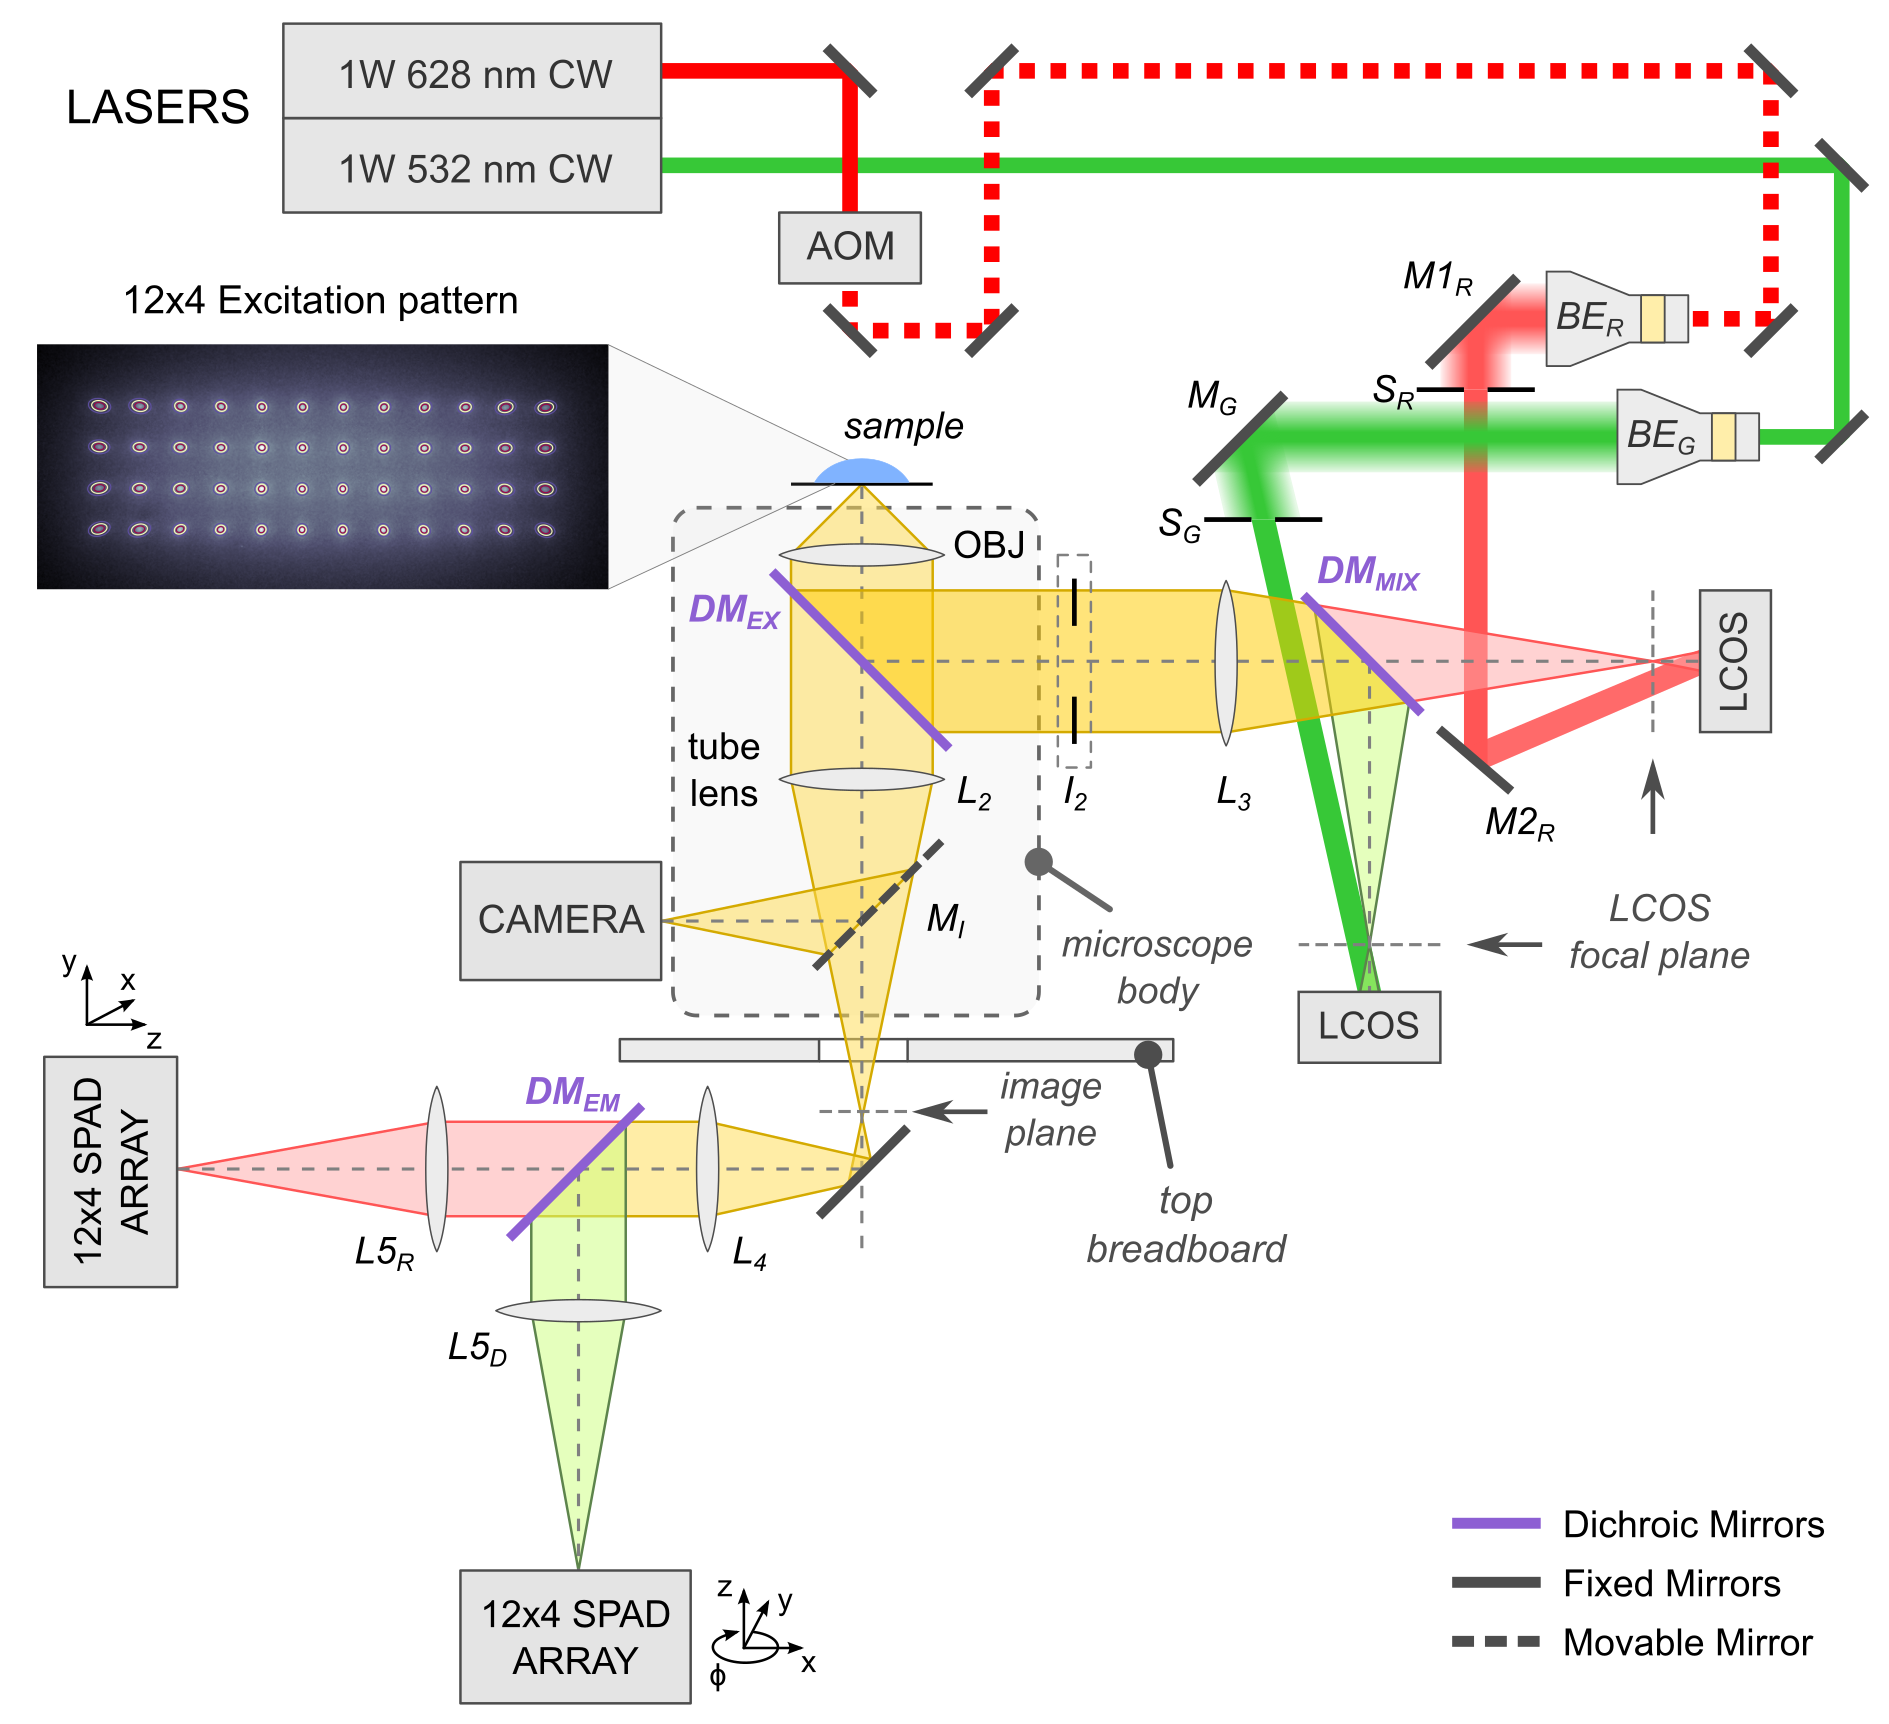
\includegraphics[width=0.7\textwidth]{figures/design_multispot_LCOS_camera_SPAD}
\caption{{\label{fig:setup} Schematic of the 48-spot smFRET-PAX setup. See
section~\ref{sec:setup} for a detailed description.}}
\end{figure*}

The setup (Fig.~\ref{fig:setup}) comprises two excitation CW lasers at
532~nm and 628~nm (2RU-VFL-Series, MPB Communications Inc., QC, Canada).
For each laser, a half-waveplate and polarizing beam splitter are used
for polarization and intensity control, as the polarization orientation
needs to be aligned along the direction required by the LCOS-SLM. The
628 nm laser is directed through an acousto-optical modulator (P/N 48058
PCAOM, electronics: P/N 64048-80-.1-4CH-5M, Neos Technology, Melbourne,
FL, USA) used for {\microsec} time-scale modulation, while the 532~nm
laser is unmodulated.
Each laser goes through a first beam expander (Keplerian
telescope, doublet lenses: 50~mm and 250~mm focal lengths). Two periscopes
bring the beams to a raised optical breadboard where a microscope body
(X71, Olympus Corporation, Japan) is fixed with its bottom port sitting
over a circular aperture. Past the periscope, each beam goes through a
second adjustable beam expander (3X, P/N 59-131, Edmund Optics Inc.).
The red laser is reflected off mirrors $M1_R$ and
$M2_R$ and phase-modulated by the ``red'' LCOS-SLM (P/N
X10468-07, Hamamatzu, Japan), before passing through the dichroic mirror
$D_{MIX}$. The green laser is reflected off $M3$,
phase-modulated by the ``green'' LCOS-SLM (P/N X10468-01, Hamamatzu),
and combines with the red excitation via the dichroic mirror
$D_{MIX}$ (T550LPXR, Chroma Technology Corp, VT, USA). Both
beams are recollimated by the $L3$ lens (f=250~mm,
AC508-250-A, Thorlabs) and focused into the sample by an high-NA
objective lens (UAPOPlan 60x, NA 1.2, Olympus) after being reflected off
the excitation dichroic mirror $DM_{EX}$ (Brightline
FF545/650-Di01, Semrock Inc., NY, USA). The excitation pattern forms a
dual-color 12x4 array of spots into the sample matching the geometry of
the two SPAD arrays. The fluorescence emission is collected by the same
objective lens, passes through the excitation dichroic
$DM_{EX}$ and is focused by the microscope tube lens either on
the side or the bottom port of the microscope. The side port mounts a
sCMOS camera (Grasshopper3 GS3-U3-23S6M-C, FLIR Integrated Imaging
Solutions Inc., BC, Canada) used during alignment while the bottom port
redirects the beams toward the emission path. Here, a relay lens
$L4$ (f=100~mm, AC254-100-A, Thorlabs) recollimates the
image and sends it to an emission dichroic mirror $D_{EM}$
(Brightline Di02-R635, Semrock), which splits the signal into a donor
(D) and acceptor (A) spectral bands. The D path goes through a band-pass
filter (Brightline FF01-582/75, Semrock) which removes residual 628~nm
laser leakage and helps suppressing any Raman scattering from the 532~nm
laser. Both D and A paths are refocused by lenses $L5_D$ /
$L5_A$ (f=150~mm, AC254-150-A, Thorlabs) on two 48-pixels
SPAD arrays\cite{gulinatti_48-pixel_2013} (denoted as donor and acceptor SPAD in the
following).

Both SPAD arrays are mounted on 3-axis micro-positioners. The directions
orthogonal to the optical axis (X-Y) are software-controlled via open-loop
piezo actuators
(actuators: Newport 8302; drivers: Newport 8752 \& 8753; Newport
Corporation, Irvine, CA, USA). The third axis (Z) has manual actuators
since the requirements on the Z directions are much less stringent than
for the X-Y directions. The donor SPAD array has an additional stage for
rotation about the optical axis, used to match the relative orientation
of the SPAD arrays.

Each SPAD arrays is equipped with an USB 2.0 connection for low-resolution
% * <michalet@chem.ucla.edu> 2017-06-16T17:36:19.581Z:
%
% > equipped with an USB 2.0 connection
% it's more than that. Maybe Polimi can expand a bit?
%
% ^ <michalet@chem.ucla.edu> 2017-06-19T18:38:35.719Z.
time-binned counting and humidity control.
In addition, a standard SCSI connector
includes 48 independent outputs providing a pulse for every detected
photon in each pixel~\cite{gulinatti_48-pixel_2013}. The two SCSI ports are fed
through a custom adapter to an FPGA-based acquisition board (FPGA board:
PXI-7813R, rack: PXI-1000B, National Instruments, Austin, TX) which
performs timestamping with 12.5~ns resolution in parallel on the 96
channels (task implemented in LabVIEW 2011 using the FPGA Toolkit). The
board transfers the data asynchronously to a host PC via an MXI-4 link
to a custom acquisition program written in LabVIEW 2011 (MXI-4 link:
rack board PXI-8331; PC board PCI-8331, National Instruments). The
acquisition program also controls the red laser alternation using a
pulse generation board (PXI-6602, National Instruments), whose clock is
synchronized with the timestamping FPGA board (PXI-7813R) through the
common bus line on the rack (PXI-1000B).

In addition to the aforementioned acquisition program, the host computer
runs a second LabVIEW 2011 program controlling the phase pattern on the
two LCOS-SLM. During alignment the acquisition program communicates with
the LCOS-control program to scan the positions of the LCOS pattern and
assess the position of the SPAD arrays (see section XXX).

The raw binary data is saved together with a text-based metadata file
containing measurement details that are used to create the final
Photon-HDF5 file\cite{ingargiola_photon-hdf5:_2016}. Once the measurement is saved on the
host PC, the raw data is immediately transferred to a linux-based
workstation via 1~Gb Ethernet link. The second workstation automatically
performs conversion to Photon-HDF5 and data analysis, leaving the host
PC available for acquiring the next set of data.


\subsection{Detectors}
\label{sec:detectors}

The current 48-spot setup employs two identical 12x4-pixel SPAD arrays whose
architecture and performance has been presented in~\onlinecite{gulinatti_48-pixel_2013}.
Here we only describe the most salient features.
The active area of each pixel has a 50~{\micron}
diameter. The array comprises 4 rows of 12 pixels (4x12) with a 500~{\micron} pitch in
% * <michalet@chem.ucla.edu> 2017-06-17T21:48:12.414Z:
%
% > pitch
% Somewhere, we need to translate this into spot separation in the sample plane
%
% ^ <michalet@chem.ucla.edu> 2017-06-19T18:38:33.005Z.
each direction.
The photon detection efficiency (PDE) reaches a maximum of $\sim$45\%
at around 550~nm\cite{gulinatti_48-pixel_2013}.

48-spot smFRET-PAX results were compared to state-of-the-art single-spot
{\usalex} setup previously described in~\onlinecite{ingargiola_multispot_2017}.
This setup employs two single-pixel commercial SPADs
(SPCM-AQRH, Excelitas Technology Corp., Waltham, MA, USA)
characterized by similar PDE as our SPAD arrays in the D spectral band but two-fold higher PDE
% * <michalet@chem.ucla.edu> 2017-06-16T00:03:05.421Z:
%
% > two-fold
% I believe this is more.
%
% ^ <michalet@chem.ucla.edu> 2017-06-19T18:38:30.183Z.
in the A spectral band.
For this reason, the {\usalex} setup is expected to be
at least twice as sensitive in the A-channel than the 48-spot setup.
A detailed comparison of the different SPAD technologies for single-molecule
measurements is reported in~\onlinecite{michalet_silicon_2014}.

\begin{figure}
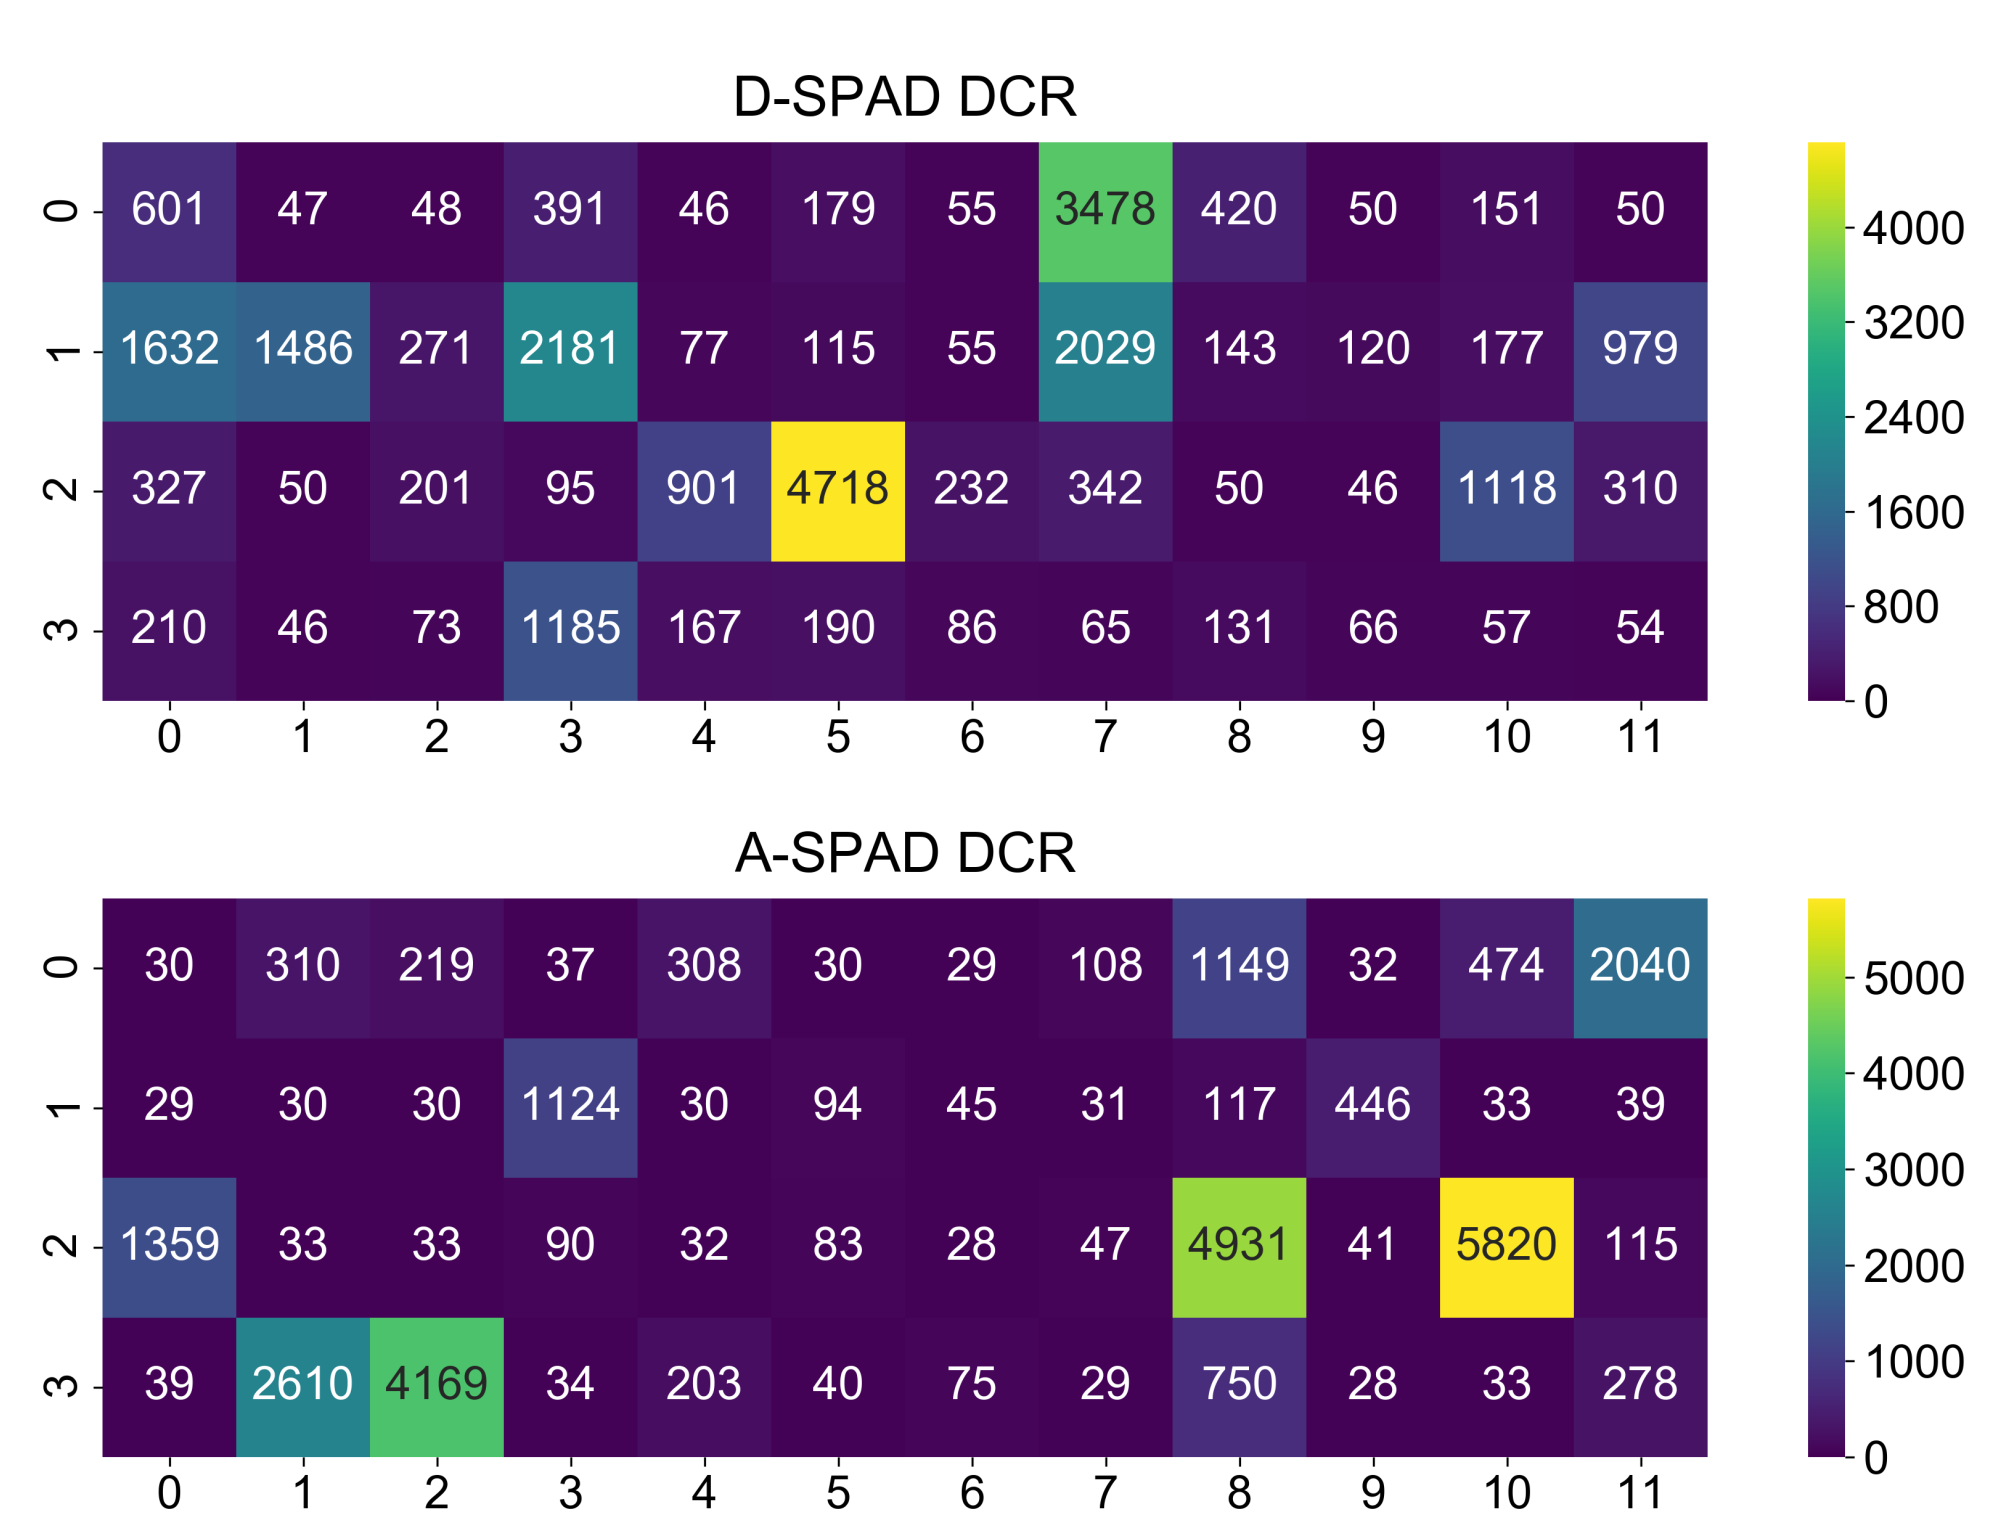
\includegraphics[width=\columnwidth]{figures/DCR-comp}
\caption{{\label{fig:dcr} Heatmaps of Dark Counting Rates (DCR) of the two 12x4
SPAD arrays (D and A) used in the current 48-spot smFRET-PAX setup.
DCR values are overlaid on each pixels. All values are in cps.
More details and the data underliyng this figure can be found in the
\href{https://github.com/48-spot-paper-analysis}{48-spot-paper-analysis}.}}
\end{figure}

\subsection{LCOS-SLM Modulation}
% * <michalet@chem.ucla.edu> 2017-06-19T18:38:04.163Z:
%
% > Modulation
% Be consistent with capitalization throughout
%
% ^ <michalet@chem.ucla.edu> 2017-06-19T18:38:26.023Z.
\label{sec:lcos}

The array of 48 excitation spots is generated for each color by an LCOS-SLM
via phase modulation of an incoming plane wave using an approach
previously described in~\onlinecite{colyer_high-throughput_2010,ingargiola_multispot_2017}.
% * <michalet@chem.ucla.edu> 2017-06-16T17:38:21.229Z:
%
% We should mention the Delon papers I sent you somewhere around here or when characterizing the illumination pattern.
%
% ^ <michalet@chem.ucla.edu> 2017-06-19T18:38:23.311Z.
The LCOS-SLM phase-pattern
implements an array of lenses that focus the spots in an image plane
at a distance of a few cm (see Fig.~\ref{fig:setup}).
The pitch of the lenses in the red and green pattern is approximately the same
(dictated by the detector geometry). Therefore a change in focal length
determines a change in diameter and thus NA of the LCOS-SLM lenses.
The chosen LCOS-SLM focal length differs in the green and red pattern
(32~mm for the red and 36~mm for the green)
in order to reduce the difference in PSF sizes between green and red excitation.


\section{Laser alignment}\label{sec:laseralign}

Each of the two lasers needs to be aligned in order
to ensure (a) maximum uniformity between spots intensities
(b) minimal aberrations across the patterns. To achieve (a) the Gaussian
laser beam is expanded so that only the central part of the beam covers
the excitation pattern (which has a maximum extension of 5~mm). To ensure
(b), the geometrical center of the pattern needs to be placed on the
optical axis.

In addition, (c) the excitation pattern of the two laser need to be
aligned so that, for each spot, there is a maximum overlap between D
and A excitation volumes.

\subsection{Individual laser alignment}

The 3X monolithic beam expanders have an adjustment ring used to control
the beam collimation. A simple way to ensure beam collimation is by sending
the beam into the microscope through the excitation dichroic mirror, removing
the external recollimation lens $L3$ and the objective
lens, while placing a mirror on the sample holder and using the LCSO-SLM
as a mirror (i.e.~with a constant phase pattern). Using the camera on
the microscope output port, we adjust the collimation until a tight spot
is formed. After adjusting the collimation, each beam needs to be
aligned so that the peak intensity is at the center of the optical axis.
To this end, without the recollimating lens $L3$, an iris
$I2$ is placed before the beam enters the microscope side
port. Using an aperture of 1-2 mm, only a narrow beamlet goes through
the objective and generates a spot from the cover-glass reflection. Only
when the input beam is parallel to the optical axis, the spot is in the
center of the field of view, assumed to be located with the center of a
cross-hair in the microscope's eyepiece.
In order to make the input beams parallel to the
optical axis, the last mirrors before the microscope is adjusted
($M2_R$ for the red and $DM_{MIX}$ for the green
laser). By defocusing the spot, we obtain symmetrical concentric patterns
only if the input beamlet intersects with the optical axis at the back
aperture of the objective lens. Since the direction is already fixed, we
move the $I2$ iris to obtain the most radially-symmetric
defocused pattern. In this way the beamlet that goes through
$I2$ coincides with the microscope optical axis. The last
steps is laterally translating the input beams (without changing the
incidence angle) in order to place the intensity peak on the iris
center. Alignment of beam direction and iris need to be repeated until
convergence. Once done, both beams are (to a good approximation)
parallel and concentric with the optical axis. When placing
$L3$ a spot is formed at a different focus position.
$L3$ can be aligned assuring that this new spot is a the
same position of the spot obtained without $L3$.

\subsection{Achieving overlap of the green and red
patterns}

Starting with the green LCOS-SLM, we project a multispot pattern into a
highly concentrated solution of dyes (100~nM - 1~\textgreek{μ}M) used for alignment.
Using a square grid of spots with an odd number of spot per side
(i.e.~9x9) ensures that one spot is at the center of the pattern. The
camera on the side-port detects an image of the pattern. The centering
of the pattern with respect to the optical axis can be assessed from the
amount of geometrical aberrations in the lateral spots. We center the
excitation pattern by rigidly translating the pattern on the LCOS-SLM so
that geometrical aberrations are roughly equivalent on the four sides.
Next, we perform a 2-D Gaussian fitting of each spot, and from the
distribution of sigmas and rotation of each Gaussian we estimate a more
accurate position of the the optical axis (analysis performed with
notebook XXX). This step may be repeated a few times until convergence.
From this point on, the X-Y positions of the green LCOS-SLM is not
changed anymore and its center becomes a reference for the optical axis
position.

Next, we activate the red LCOS-SLM and project a multispot pattern
excited by the 628~nm laser. Using the camera we align the red pattern to
the green one used as reference. A first coarse adjustment of the red
LCOS-SLM pattern is manually performed by looking at the emission
pattern on the live camera display. Then, the center position of the red
LCOS-SLM pattern is finely adjusted by fitting the spot positions in the
green and red images (Fig. \ref{fig:patternfit}), taken separately (the
analysis notebook can be found in
\href{https://github.com/multispot-software}{multispot-software}).

Finally, in order to reduce the background due to unmodulated light, two
custom-made rectangular slits (aluminum with black finish) are added in
the path before each LCOS. The slits are aligned to illuminate only the
12x4 pattern ($\pm$1~mm) on the LCOS-SLM.

\begin{figure}
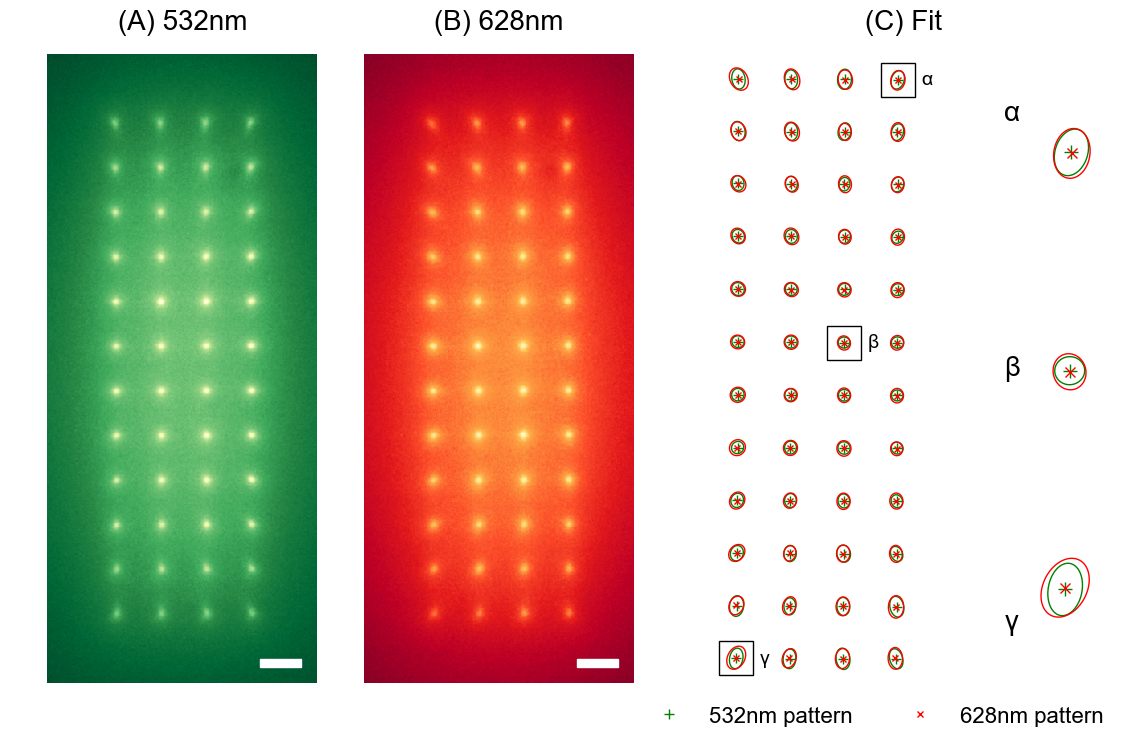
\includegraphics[width=\columnwidth]{{figures/2017-04-28_conf9_G_conf14_R_green_red_pattern_and_fit}}
\caption{{\label{fig:patternfit}
The 12x4 multispot pattern for green (A) and red (B)
excitation and Gaussian fit of the spots (C). The pattern is acquired by
a camera on the microscope side port (see fig.~\ref{fig:setup}) using a
solution of ATTO550 and ATTO647N at high concentration ($\sim$100~nM).
Emission due to 532~nm and 628~nm laser is acquired with two subsequent
acquisitions and reported in false-colors in panels (A) and (B).
Scale bars are 5~{\micron} long.
To assess the alignment,
each spot in the two images is fitted with a 2D Gaussian function. Panel
(C) reports an overlays of the fitted peak positions peak positions and
contour of the Gaussian waist for 532~nm (\emph{green}) and 628~nm
(\emph{red}) images. A zoom-in for 3 representative spots is reported on
the right. The elliptical shape of the Gaussian and their rotation is
due to geometrical aberrations.%
}}
\end{figure}

\section{SPAD arrays alignment}\label{spad-alignment}

Both detectors must be aligned so that each pixel is optically
conjugated to the corresponding excitation volume (excitation PSF). The
goal is having pairs of corresponding pixels on the two arrays,
detecting photons from the same volume in the sample (detection PSF). At
the same time, in order to maximize the signal, the detection PSF needs to be
concentric with the excitation PSF. Achieving this with a 2-D
arrangement of spots and pixels requires not only aligning the X-Y
position of the detectors (as in single-spot measurements) but also
aligning the relative rotation of the two SPADs and adjusting the pitch
and rotation of the excitation pattern to optimally match the detectors'
geometry.

For alignment we use a high concentration dye mixture (ATTO550,
ATTO647N, $\sim$500~nM) excited by both lasers.
With this sample, the 532~nm laser generates fluorescence signal in both D and A
channel, while the 628~nm laser only generates signal in the A channel.
At this point, the center of the both 532~nm and 628~nm excitation patterns
has already been fixed in order to minimize geometrical aberrations
as described in section~\ref{sec:laseralign}.
Therefore, the excitation pattern position is used as the reference
to which aligning the SPAD arrays.
Starting with the green laser only, both SPADs are manually positioned
in X and Y to match the center of the excitation pattern. This is achieved
by maximizing timetraces of SPAD counts (displayed by the acquisition
program) while moving the detectors.

Next, we perform a more automated procedure for fine alignment called in
the following ``multispot scan''. A multispot scan involves rigidly
translating a multispot pattern (typically 4x4 spots) on a LCOS-SLM in
discrete steps along a cross path.
At the same time, counts from a SPAD
array are integrated for each pattern position for 300~ms.
During a scan, each emission spot draws a cross path roughly centered
on a SPAD's pixel.
A typical scan covers a range of 10 LCOS-SLM pixels with a step of 0.4
and is performed sequentially in X and Y directions.
The acquired counts as a function of the LCOS-SLM position resemble a peak
profile that is used to estimate SPAD's pixel positions in LCOS-SLM
coordinates. Averaging the SPAD pixel positions we obtain an accurate
estimation of the SPAD array's center. Ultimately, this procedure yields
the offset of each SPAD array with respect to the ideal excitation pattern
center. With this information, we move the SPAD arrays to the ideal
X-Y position using software-controlled piezo micro-positioners.
The sequence of multispot scan and SPAD array translation is repeated
until convergence.
Initially the two SPAD arrays are aligned with respect to the green
LCOS-SLM pattern (532 nm). Next, the position of the red LCOS-SLM pattern
(628 nm) is fine-tuned to match the position of the A SPAD array (the D
SPAD array does not detect any signal with 628 nm excitation). The
optimal position of the red excitation pattern is determined from a
multispot scan performed with the red LCOS-SLM while counts are acquired
with the A SPAD array. After this, both red an green excitation
patterns, and D/A SPAD array positions are fixed and the alignment is
complete.

The whole fine alignment procedure is routinely performed at the
beginning of each day of measurements and requires about 30 minutes.

\subsection{Rotation and pitch
adjustment}\label{rotation-and-pitch-adjustment}

In the previous section we outlined the general fine-alignment procedure
repeated daily when using the multispot setup. However, when
building the setup, additional steps are
necessary (a) to align the relative rotation of the two SPAD arrays, (b)
to determine the best pitch in X and Y for the green and red excitation
pattern and (c) to optimize the SPAD position along the optical axis
(Z).

To extract rotation and pitch information, we perform a
multispot scan followed by an additional analysis step. In particular, the
set of X-Y positions of each SPAD pixel obtained from the scan is fitted to a
rectangular grid.
The fitted grid parameters are: center position, pitch in X, pitch in Y and
rotation angle. Each SPAD array will have a different set of fitted
parameters.

To adjust the rotation angle, one of the SPAD arrays (D) is
rotated about the optical axis in order to minimize the difference in
rotation angle between the two SPAD arrays as obtained from the scan
fits. Once the orientations of two SPAD arrays matches, the rotation
stage is locked, ensuring long-term stability of the rotational angle.

Regarding the pitch, the information from the scan fits is used to
determine the X and Y pitch of the LCOS-SLM pattern that optimally
matches both SPAD arrays. We observed X and Y pitch difference of 1-2\%
due to non-idealities (stigmatism) in the optical path.

\textbf{Figure}: scatter plot of center positions for: D-SPAD G laser,
A-SPAD G laser, A-SPAD A laser.

\section{smFRET measurements}\label{sec:smfret-meas}

\subsection{Analysis}

Single-molecule measurements were performed with 40 base-pair dsDNA samples
labeled with ATTO550 (D) and ATTO647N (A) (ATTOTEC GmbH, Heidelberg, Germany)
located at different distances.

D-A separation of 7d, 12 and 22 base pairs (7d, 12d, 22d) were used in these
experiments, as they cover the typical range of distances of interest in
single-molecule FRET.
Samples were diluted to single-molecule concentration (~50 pM) in TE50 buffer
(10~mM Tris, bring to pH 8.0 with HCl, 1 mM EDTA, 50~mM NaCl).
Full details regarding these samples are provide in ref.~\onlinecite{ingargiola_multispot_2017}.

We analyzed data using standard {\usalex} methods\cite{lee_accurate_2005}
with modifications required for smFRET-PAX\cite{doose_periodic_2007}.
The three steps of the analysis are:
(a) background estimation, (b) burst search, (c) burst selection.
Background estimation, which is used to correct the burst counts
in the different photon streams, was performed in 10~s time windows
in order to account for possible variations during the measurement.
Burst search was performed independently for each spot
using the sliding-window algorithm~\cite{fries_quantitative_1998}
and a constant-rate threshold for all spots~\cite{ingargiola_fretbursts:_2016}.

The main result of the {\usalex} analysis is a so-called E-S histogram,
a 2-D histograms where each bursts is represented by a
pair of values $(E, S)$. $E$ is either the FRET efficiency or, more commonly,
the uncorrected FRET efficiency known as proximity ratio, $E_{PR}$.  $E_{PR}$
is easier to compute
and provides an approximation suitable for identifying sub-populations.
However, when the purpose is to extract D-A distances (which is not the
objective of this study),
$E$ needs to be computed, requiring and accurate estimation of
all  correction coefficients.
$S$ is the "stoichiometry ratio", a quantity ideally centered around 0.5 for
doubly-labeled species, close to 0 for A-only and close to 1
for D-only species. When using the simpler version without correction
(eq.~\ref{eq:S}), $S$ can depend on $E$ and, for doubly-labeled
molecules, is only approximately centered around 0.5.
The use of the $(E, S)$ pair (corrected or uncorrected)
allows separating singly- and doubly-labeled species and, within the
doubly-labeled ones, distinguishing FRET sub-populations.

In this paper, we report proximity ratios $E_{PR}$ computed according to
eq.~\ref{eq:Epr}, and a ``modified stoichiometry ratio'' $S_u$ defined
in eq.~\ref{eq:Su}. $S_u$ is a variant of the classical
smFRET-PAX stoichiometry\cite{doose_periodic_2007}, which reduces the effect of
shot noise and improves the separability of D-only and FRET populations.
More details can be found in section~\ref{sec:alex_pax}.
Note that, in all this work, the results of two spots (the two leftmost
spots in the second row) are missing,
because of an active quenching circuit (AQC) failure in the D-SPAD array.

\subsection{Peak photon rate}

\begin{figure*}
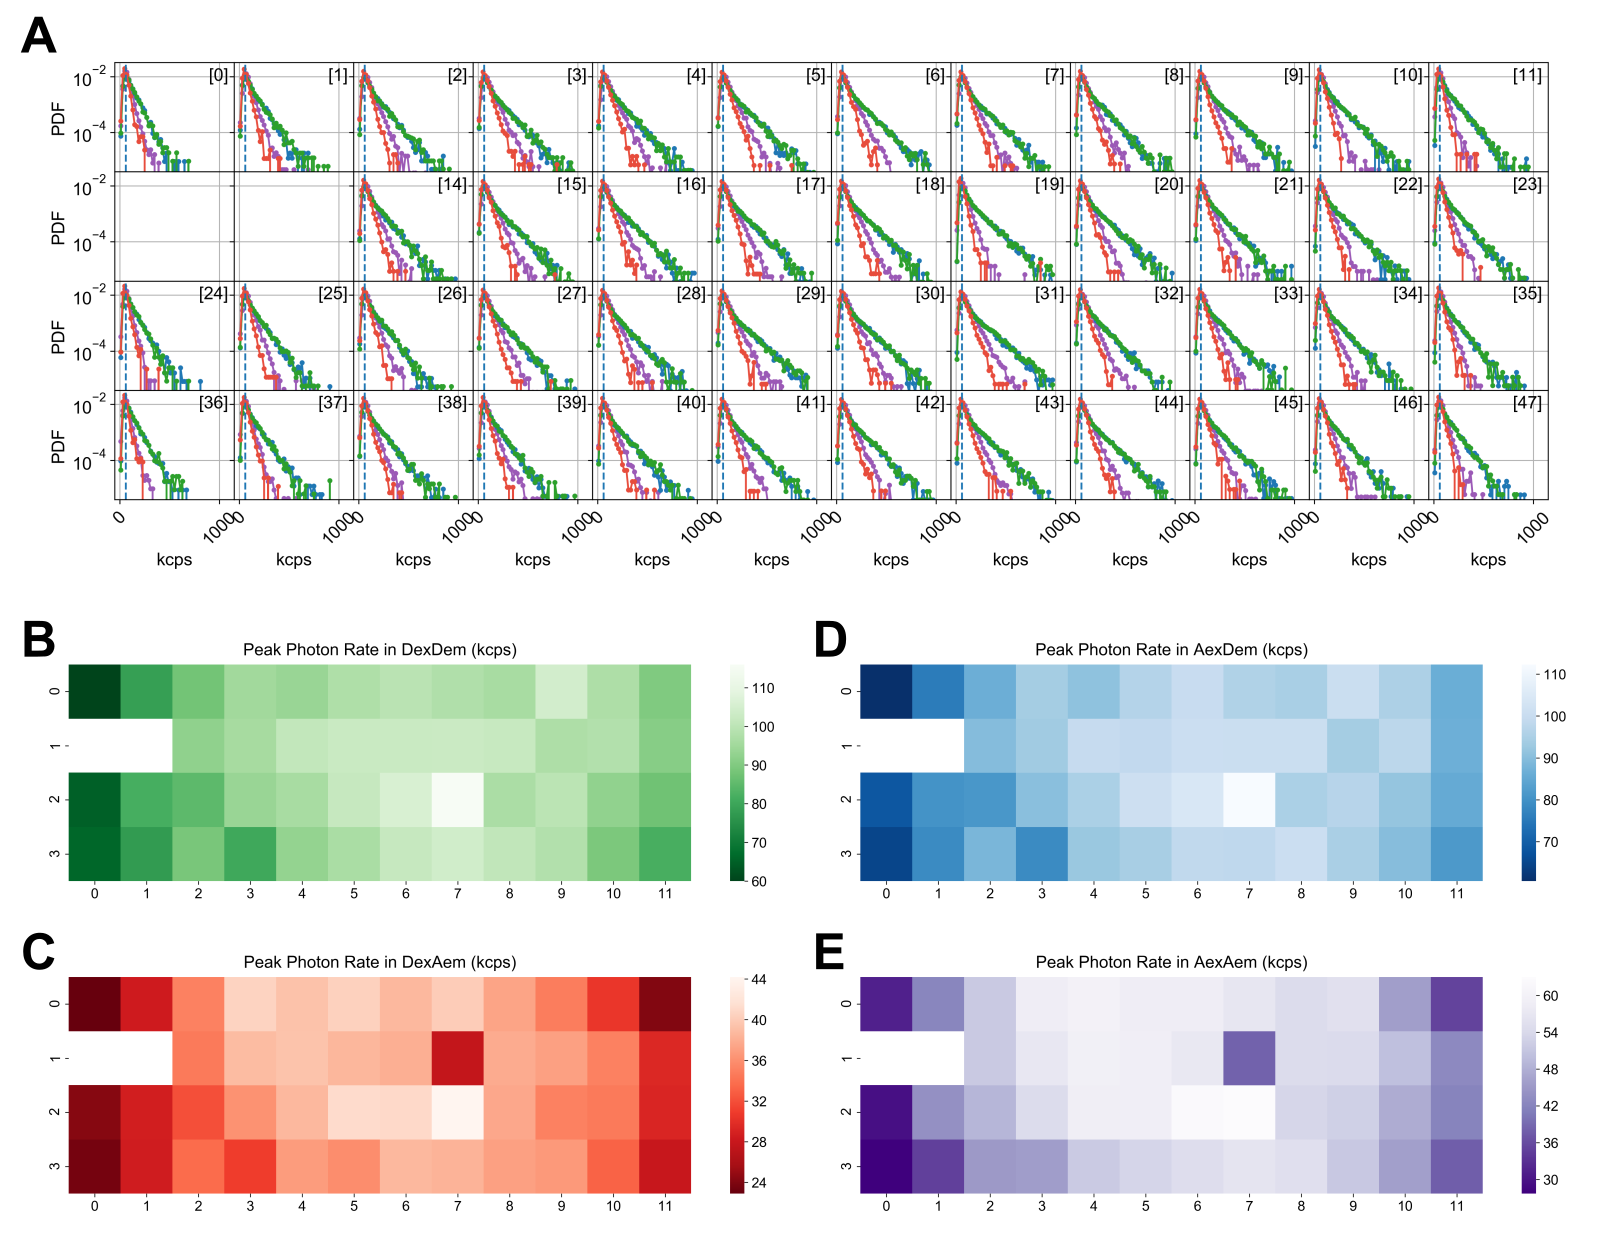
\includegraphics[width=\textwidth]{{figures/phrates_composite}}
\caption{{\label{fig:phrates48_comp}
Peak photon rate in each of the 48 spots for the 12d dsDNA sample.
Panel A: full distribution of peak photon rates. Panels
B-E: Mean of the peak photon rate distribution in the different photon
steams. Two lateral spots in the second exhibit no signal because of
two malfunctioning pixels in the D-SPAD array.
Colors indicate different photon streams.
Green $D_{ex}D_{em}$, red $D_{ex}A_{em}$, light blue $DA_{ex}D_{em}$,
purple $DA_{ex}A_{em}$.%
}}
\end{figure*}

\begin{figure}
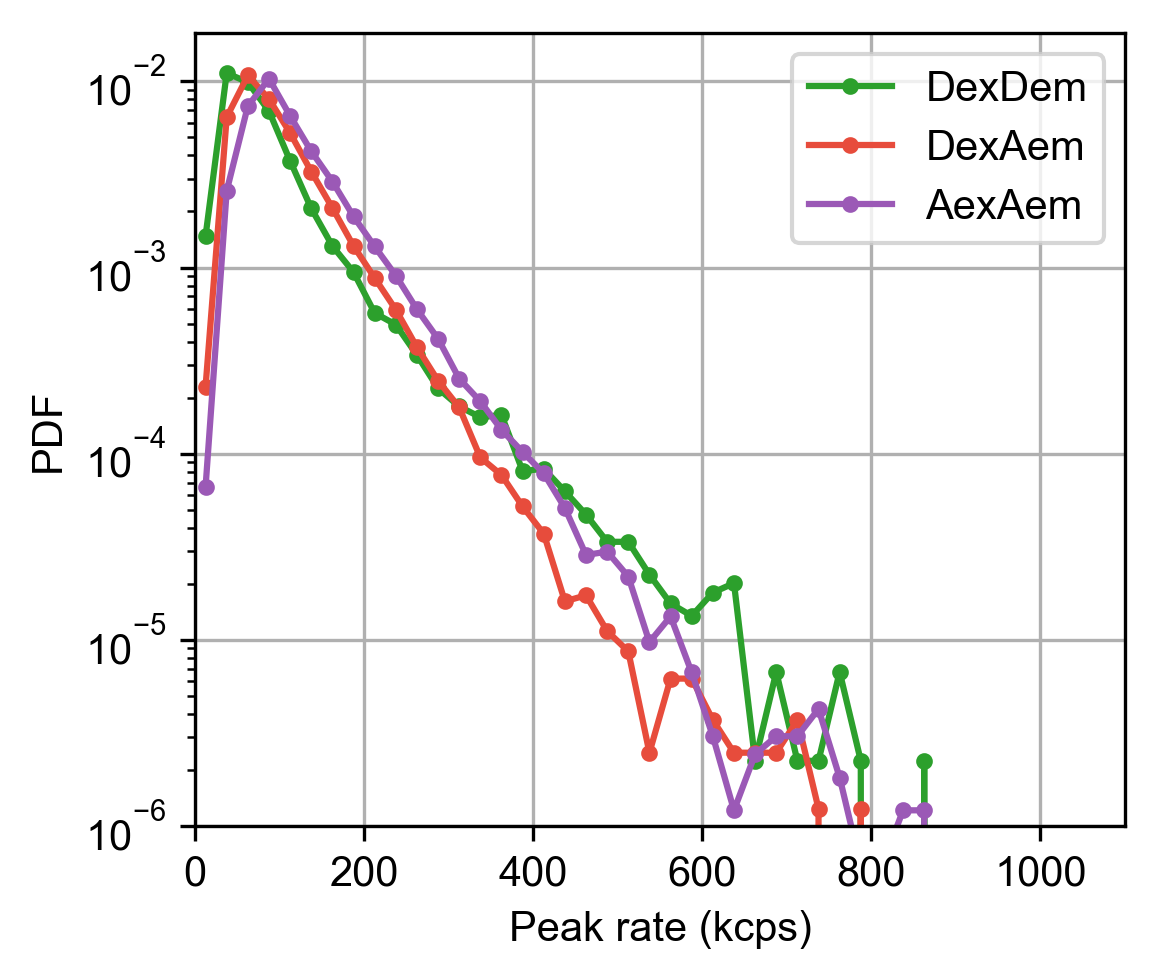
\includegraphics[width=0.8\columnwidth]{{figures/2017-06-02_002_12d_usALEX_peak_phrate}}
\caption{{\label{fig:phrates_usalex}
Distribution of peak photon rates in a single-spot {\usalex} measurement
of the 12d dsDNA sample.
Colors indicate different photon streams.
Green $D_{ex}D_{em}$, red $D_{ex}A_{em}$,
purple $A_{ex}A_{em}$.%
}}
\end{figure}

We start by analyzing the peak photon rate reached in each burst,
a quantity scaling with the peak PSF intensity\cite{ingargiola_multispot_2017}.
Fig.~\ref{fig:phrates48_comp} shows the background-corrected peak photon-rate
in each burst for the 48 spots. Panel A shows the full peak photon-rate
distributions with their characteristic exponential tails.
Panel B-E show, for the different photon streams,
heatmaps of the peak photon-rate mean values
(i.e. the decay constant of the exponential tail).
Due to the Gaussian profile of the excitation beam and to geometrical
aberrations, the lateral pixels receive a lower signal than the central ones.
As a result, the peak photon-rate decreases and a smaller number of
single-molecule bursts is detected in the lateral spots.
While this effect decreases the overall maximum reachable throughput,
it does not influence the uniformity of the ratiometric quantities
$E_{PR}$ and $S$ across the different spots.
Conversely, in Fig.~\ref{fig:phrates48_comp} (Panels C, E), we observe that pixel
at position (1, 7) in the A-SPAD arrays, systematically
detects less photons, an effect ascribed to a lower PDE of that pixel.
This effect causes a bias in $E_{PR}$ and $S$ quantities as shown below.
Furthermore, two pixels in the

Fig.~\ref{fig:phrates_usalex} shows the distribution
of peak photon rates as obtained with the {\usalex} setup.
Comparing Fig.~\ref{fig:phrates48_comp} Panel~A and~\ref{fig:phrates_usalex}
we note that the lower sensitivity in the A-SPAD array results in lower peak
photon rate in the $D_{ex}A_{em}$ (red) and $DA_{ex}A_{em}$ (purple) streams
in the 48-spot setup.

\subsection{E-S histograms}
After the initial burst search it is necessary to apply a burst selection
criterium to reject the smallest burst which dominate the distribution.
Fig.~\ref{fig:alexhist48all} shows the E-S histogram for the 12d sample,
after a burt selection obtained setting a threshold on the minimum
bursts counts obtained from photon in all the streams.
We observe that D-only and FRET populations (respectively top left corner
and center in the 2-D histogram) are clearly distinguishable in most channels.
Moreover, as shown in Fig~\ref{fig:alexhist48fret}, it is easy to isolate
the FRET population(s) by applying a burst
selection on the $DA_{ex}A_{em}$ counts and on $D_ex$ counts.
The separation of FRET from singly-labeled species is the main advantage
of the dual laser excitation.

Without any further calibration, the spread across the different channels
is limited and does not affect the ability to distinguish sub-populations.
This is evident in Fig.~\ref{fig:fittedFRETscatter} which shows the
$E_PR$ and $S_u$ peak center position in the the different spots for
both D-only and FRET populations.
Fig.~\ref{fig:fretfit48vsmean} shows, separately for each channel,
the center and $\pm1\,\sigma$ range of the fitted E-S peak
for the FRET population (blue dot and error-bar).
The orange dot is the mean center peak position
across all the channels. We note that, for almost all channels, the
deviation of the peak position is very well below the $\pm1\,\sigma$
range. One exception is channel 19, where the lower PDE of the A pixel
causes a larger deviation of the peak position.
While in Fig.~\ref{fig:fittedFRETscatter} and~\ref{fig:fretfit48vsmean}
we present results without any channel calibration for the purpose
of illustrating the raw performances of the system.
It is possible, however, to reduce the channel-to-channel variation
on E and S peak position by applying the per-channel calibration reported
in~\ref{sec:perchcorr}.

\begin{figure*}
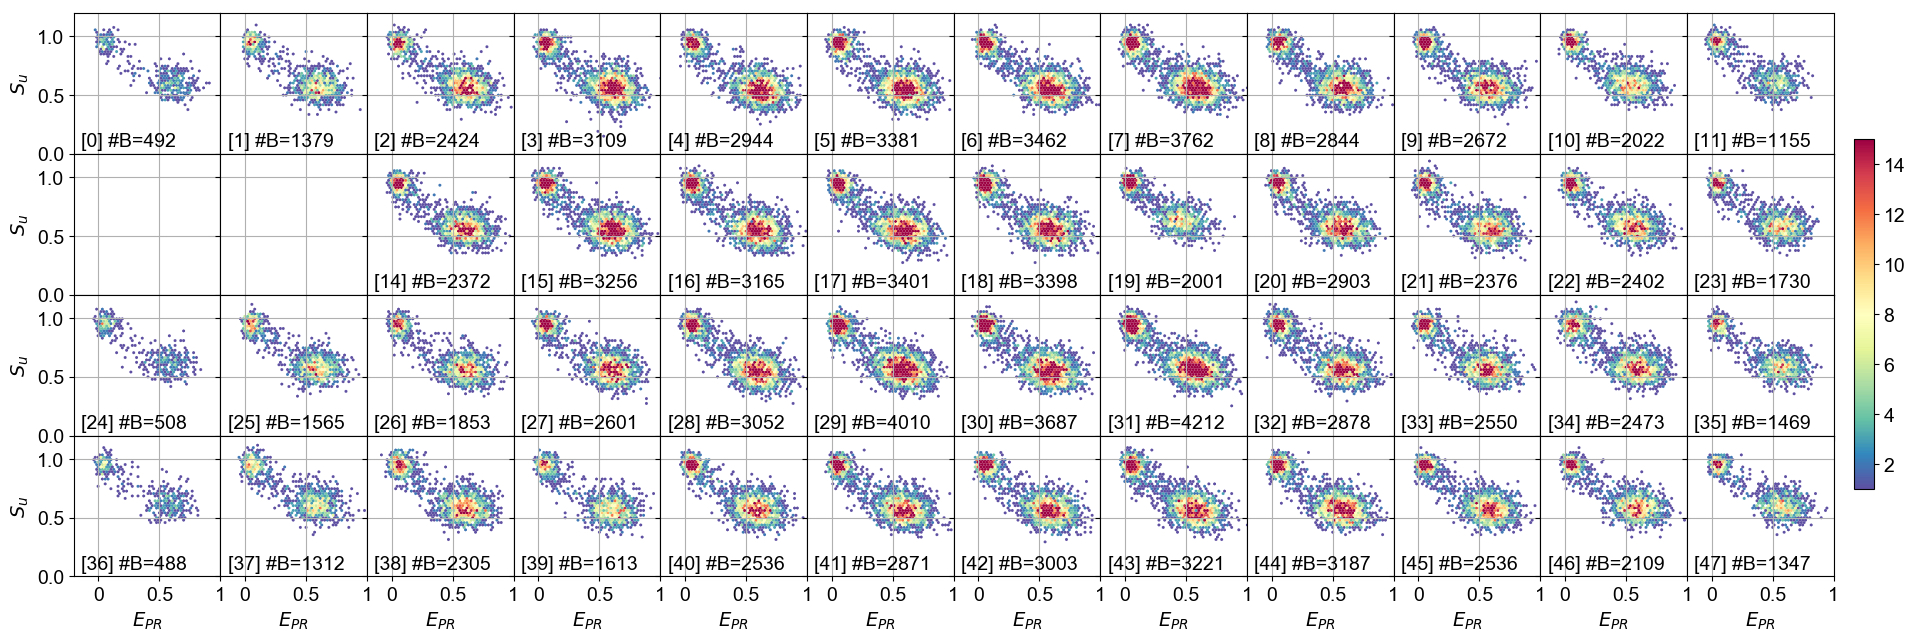
\includegraphics[width=\textwidth]{{{figures/2017-05-23_08_12d_48spot_alex_hist_Su_all-bursts}}}
\caption{{\label{fig:alexhist48all} $E_{PR}$ versus $S_u$
histograms for the different spots for the 12d dsDNA sample. Two
populations visible D-only (cluster at $E_{PR}=0$,
$S_u=1$) and FRET population (cluster at $E_{PR}=0.6$,
$S_u=0.6$). Burst search is performed on all photons with
constant-threshold burst search (50~kcps). Burst selection is performed
on the total burst size after background correction with a threshold of
40 photons. Text in each subplot reports spot number
($[\cdot]$) and number of bursts (\#B).%
}}
\end{figure*}

\begin{figure*}
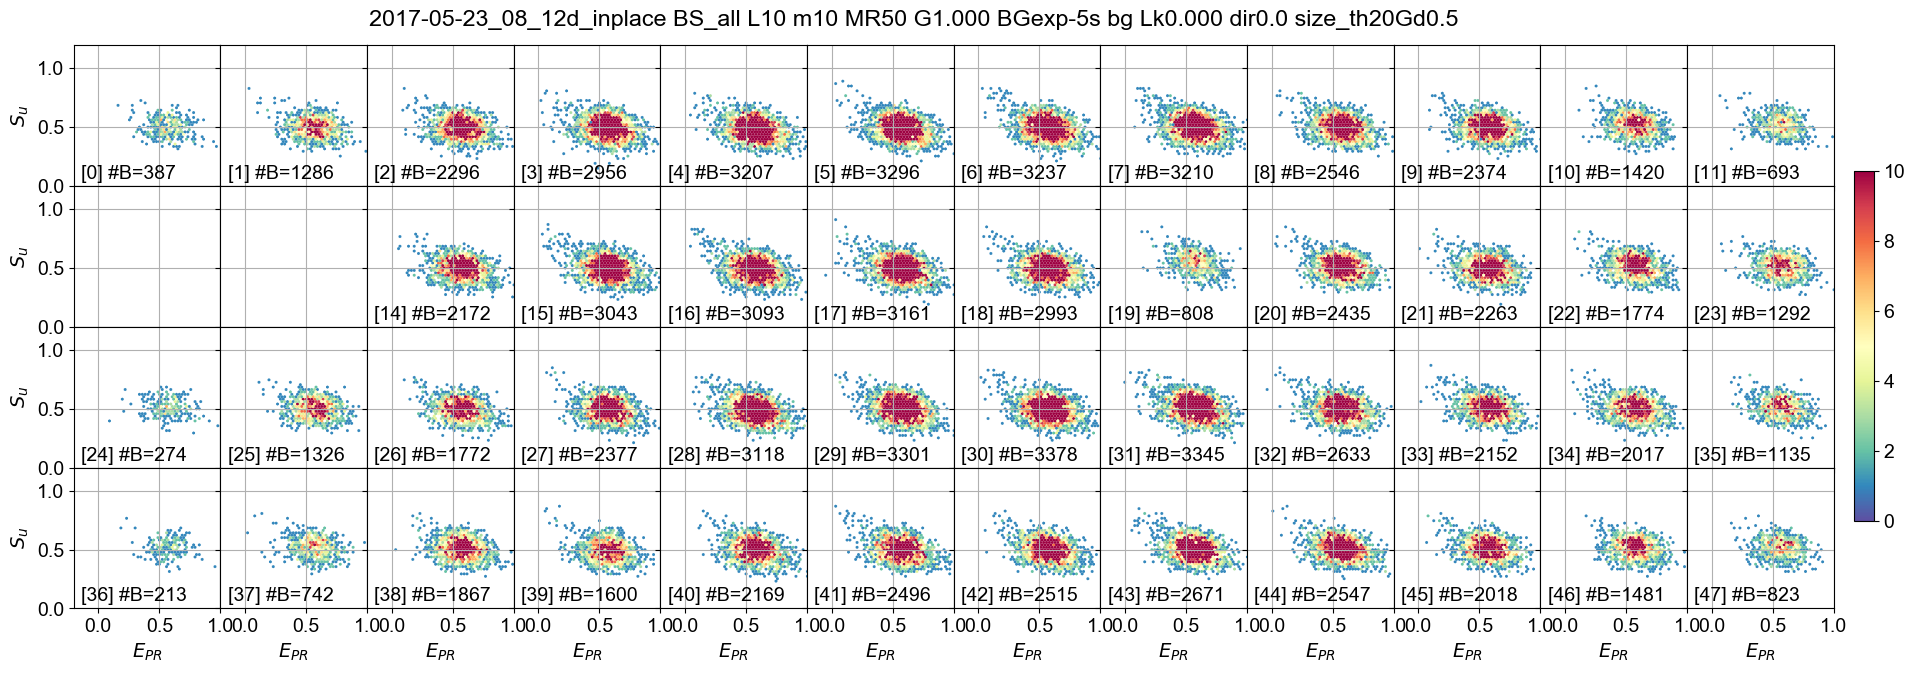
\includegraphics[width=\textwidth]{{figures/2017-05-23_08_12d_48spot_alex_hist_Su_naa_AND_size_selection}}
\caption{{\label{fig:alexhist48fret} $E_{PR}$ versus $S_u$
histograms for the different spots for the 12d dsDNA sample. Data and
burst search is identical as in figure~\ref{fig:alexhist48all}, while
burst selection has been tailored to select only the FRET population.
The burst selection criteria is the following: a burst is selected if
counts in $D_{ex}DA_{em}$ stream are larger than 20 and counts in
$DA_{ex}A_{em}$ stream are larger than 20. Text in each subplot
reports spot number ($[\cdot]$) and number of bursts (\#B).%
}}
\end{figure*}

\begin{figure}
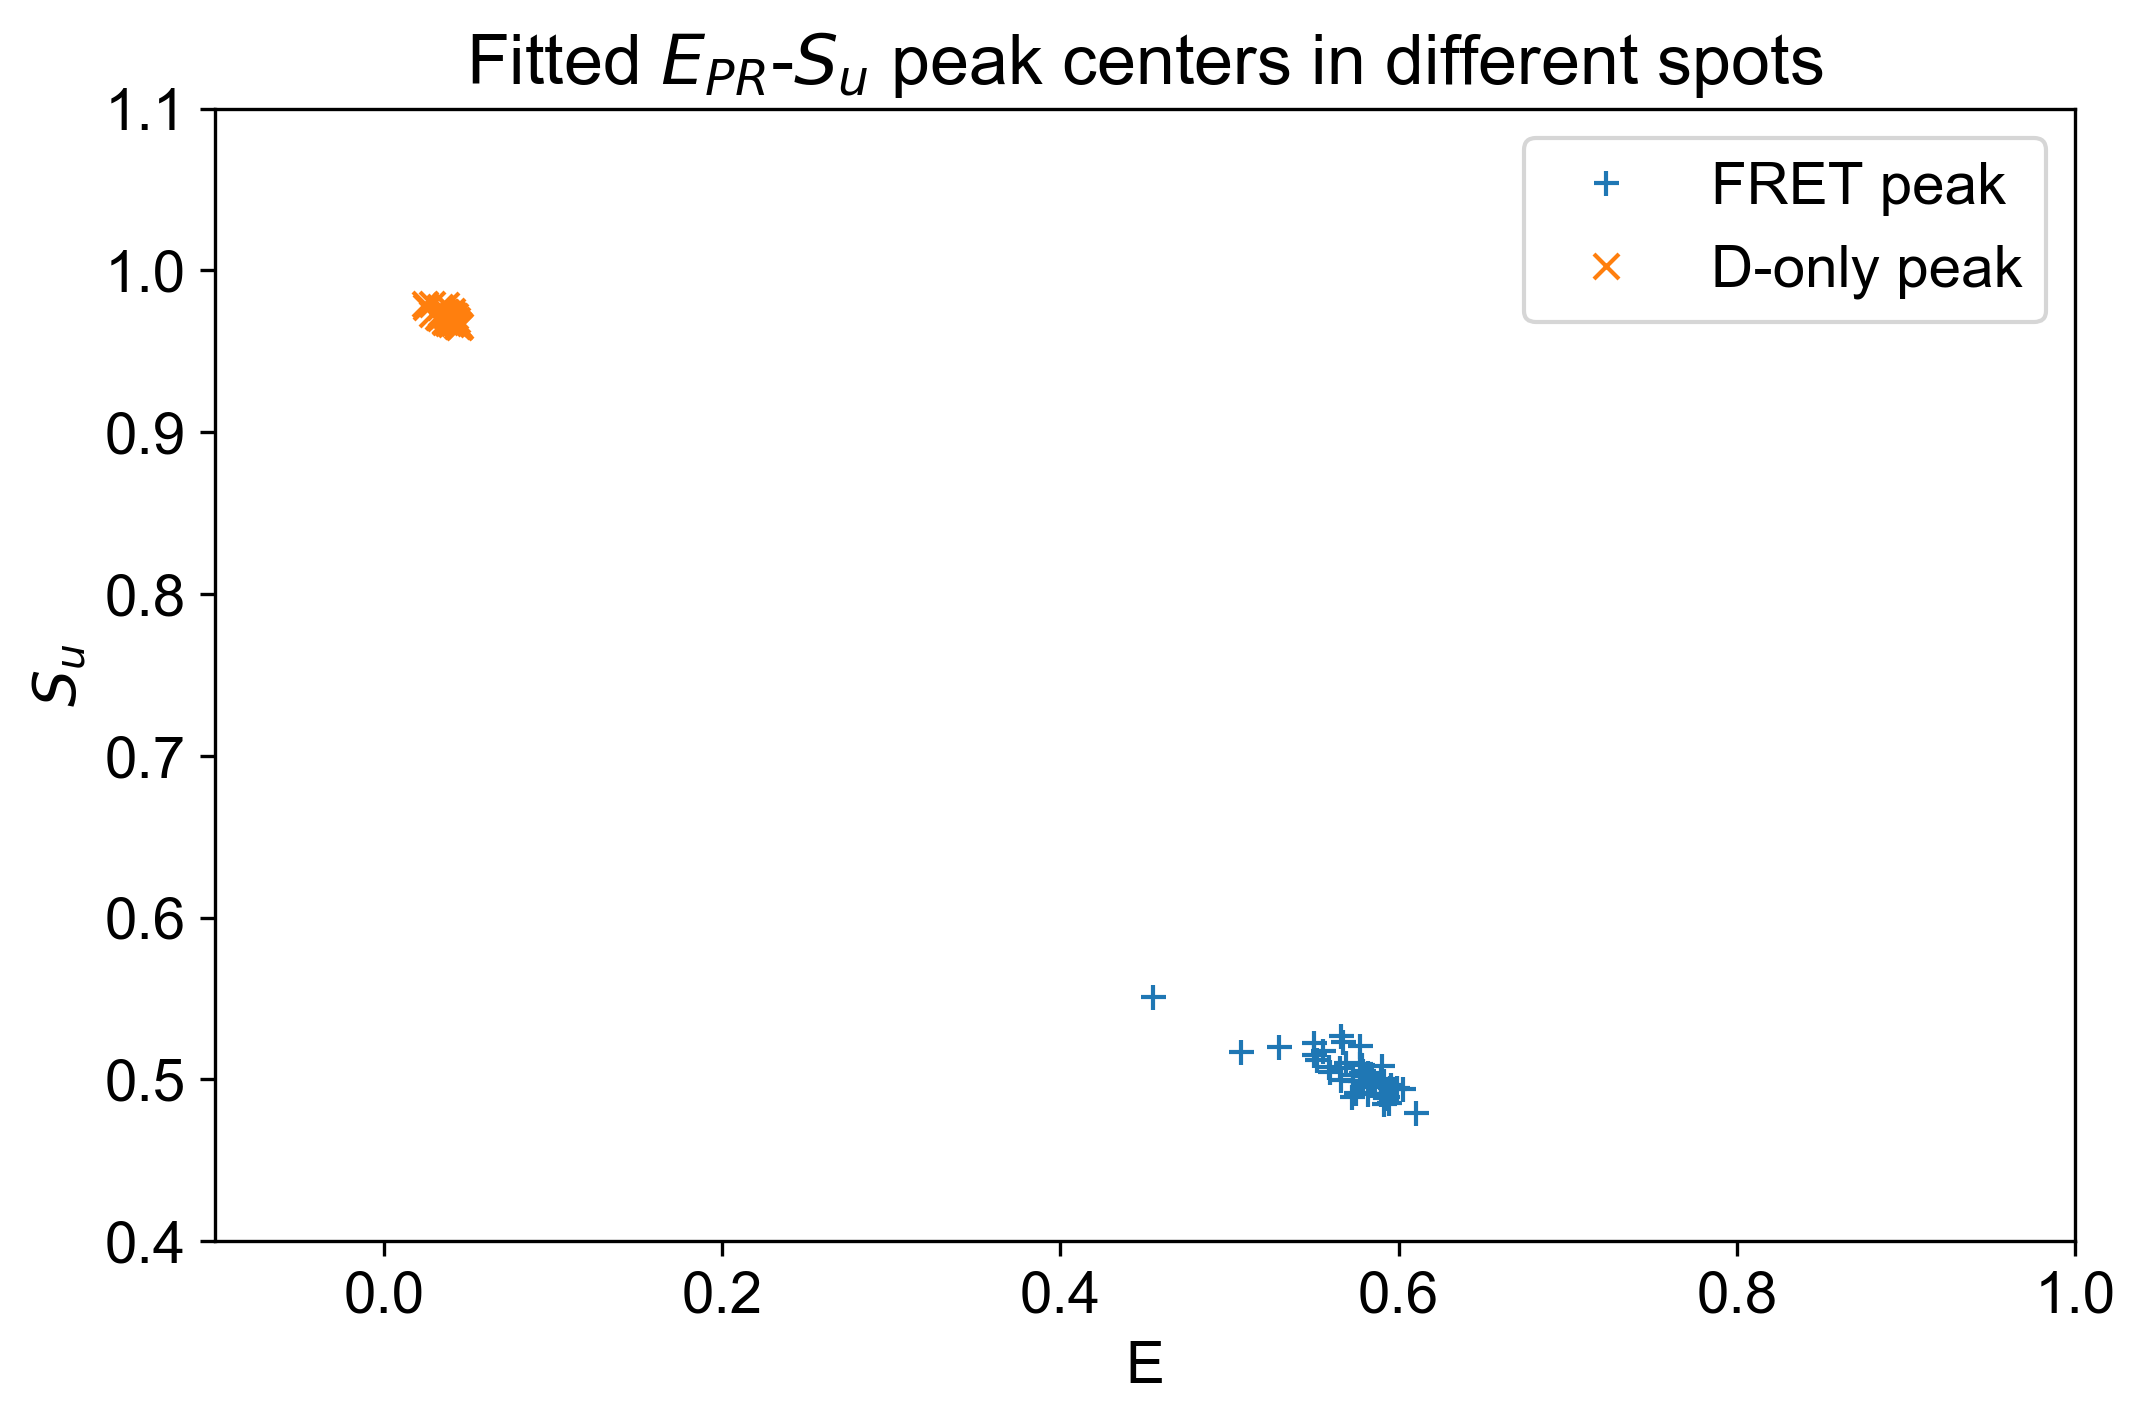
\includegraphics[width=0.8\columnwidth]{figures/2017-05-23_08_12d_FRET_vs_DO_fitted_Epr-Su_peak_position}
\caption{\label{fig:fittedFRETscatter}
Scatter plot of the fitted $E_{PR}$, $S_u$ peak
position in the different spots for the D-only (\emph{orange cross})
and FRET population (\emph{blue plus}). Values were obtained by simple Gaussian
fitting of the 1-D histogram of $E_PR$ and $S_u$ after a bursts selection
that isolated D-only and FRET populations respectively.}
\end{figure}

\begin{figure*}
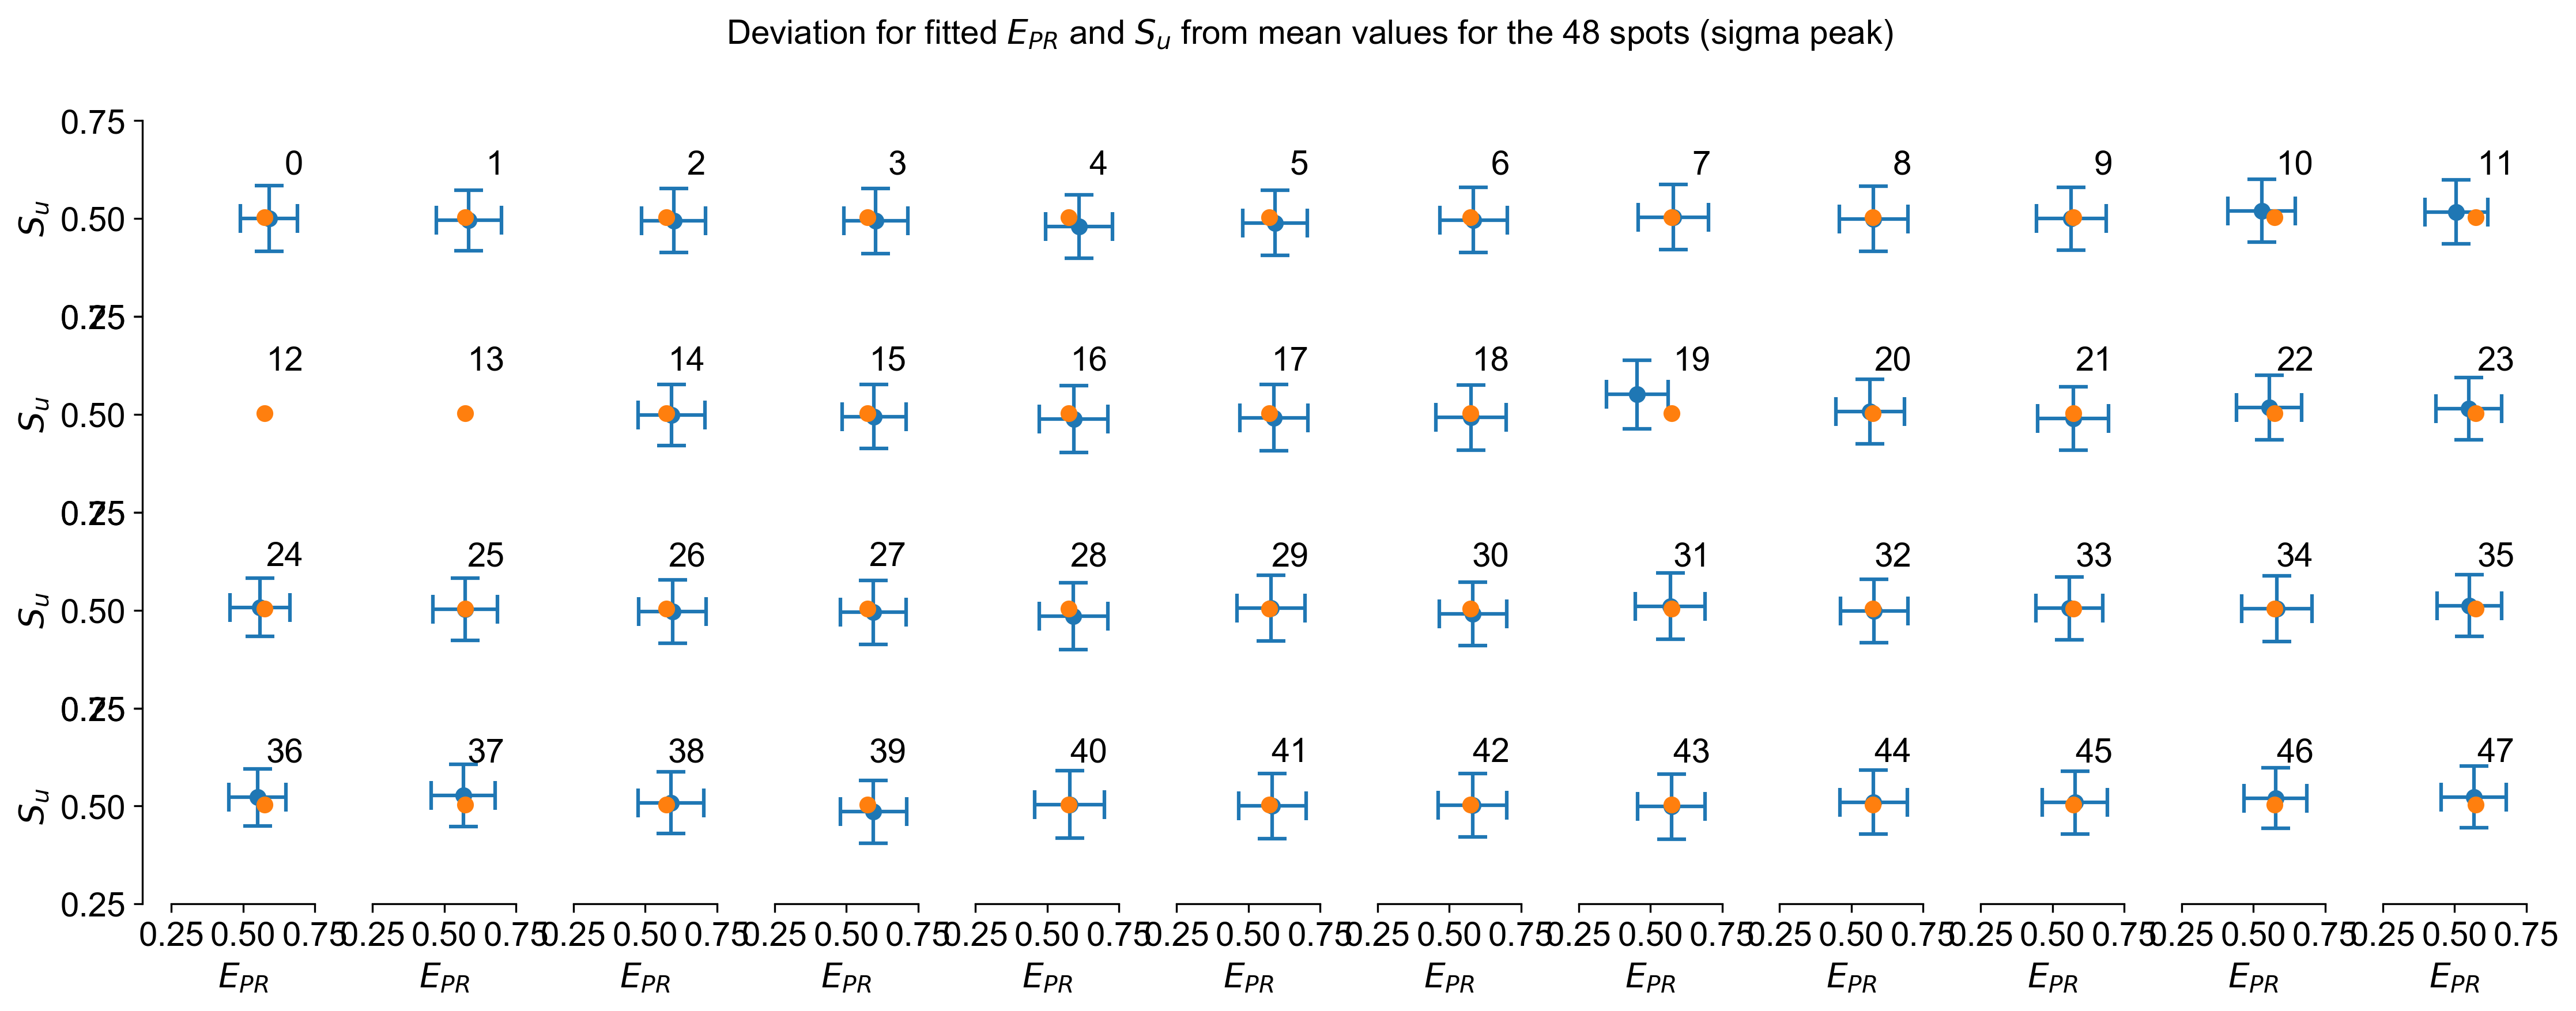
\includegraphics[width=\textwidth]{figures/2017-05-23_08_12d_48-spot_Epr-Su_peak_position_deviation_from_mean}
\caption{{\label{fig:fretfit48vsmean} Fitted FRET peak position ($E_{PR}, S_u$,
\emph{blue dots}) and $\pm 1 \sigma $ of the fitted Gaussian
(\emph{blue error bars}) for the 48 spots. As a reference, the mean
$E_{PR}, S_u$ across the 48 spots (\emph{orange dot}) is reported
in each subplot.  The spot number is indicated in the top right corner of
each subplot.%
}}
\end{figure*}


\subsection{Pooling data from all channels}
To illustrate the high-throughput performance of the 48-spot system, we
build an ALEX histogram with bursts from all channels within a 15~s window
of one measurement (Fig.~\ref{fig:alex_mspot_15}).
For comparison, Fig.~\ref{fig:alex_sspot_15} shows a similar histogram obtained
from a 15~s window during a measurement of the same sample using the
single-spot {\usalex} setup. While, we observe that
the total number of bursts  detected in the multispot measurement
is about 12 times larger than in the single spot measurement a quantitative
comparison cannot be done because the measurements were taken on different
dilutions in the two setups. Apart from the difficulty in controlling
the sample concentration with high accuracy, there are other reasons why the
burst number would not exactly scale with the number of spots.
First, in the multispot setup, it is difficult to estimate the power
in each spot because the intensity is not uniform (the lateral spots
receive less power). The power is calibrated so that, in the central spots,
we obtain a signal in the D-channel comparable to the single-spot measurements
(which used 180~\textgreek{μ}W @ 532~nm). The lateral spots receive a lower
power and therefore detect lower number of bursts.
Second, the detection efficiency of the SPAD array in the red part
of the spectrum is lower than that of the corresponding SPAD in the
single-spot setup (see section~\ref{sec:detectors}),
reducing total burst size and therefore the number of bursts selected with
a given threshold.


\begin{figure}
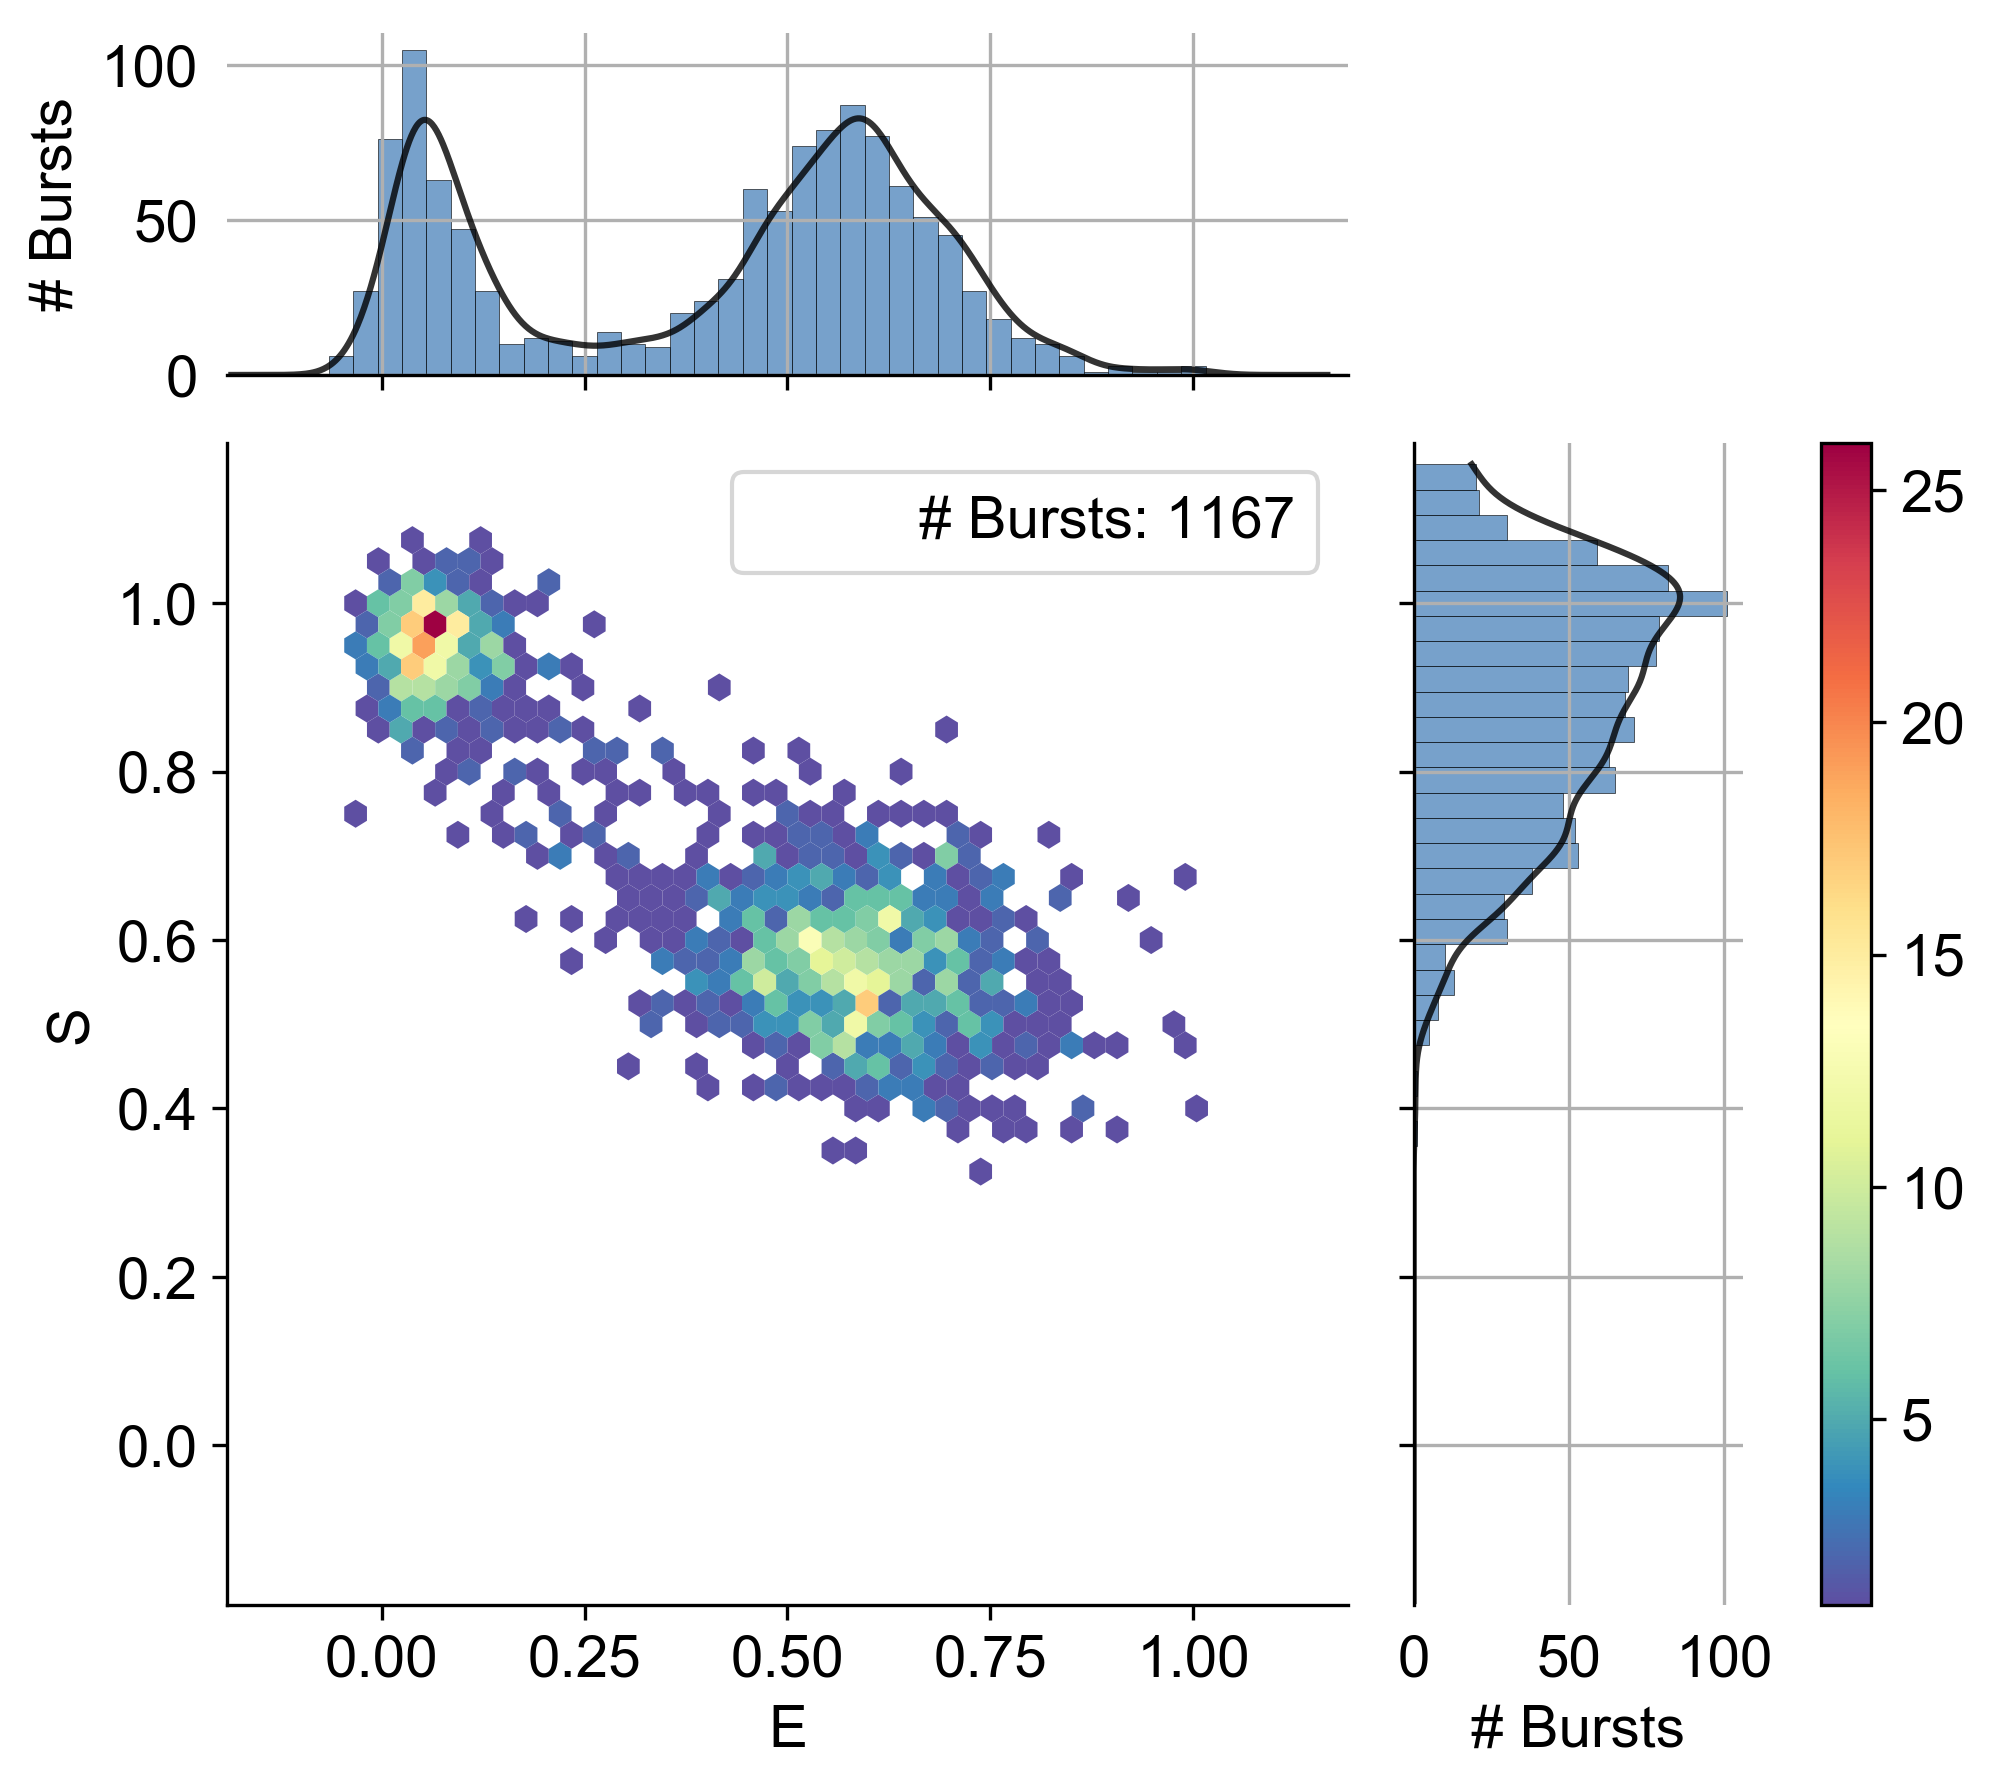
\includegraphics[width=\columnwidth]{figures/2017-05-23_08_12d_alex_jointplot_15s}
\caption{\label{fig:alex_mspot_15}
Multispot ALEX histogram obtained from 15~s of acquisition by pooling bursts
from all the 48 spots.}
\end{figure}

\begin{figure}
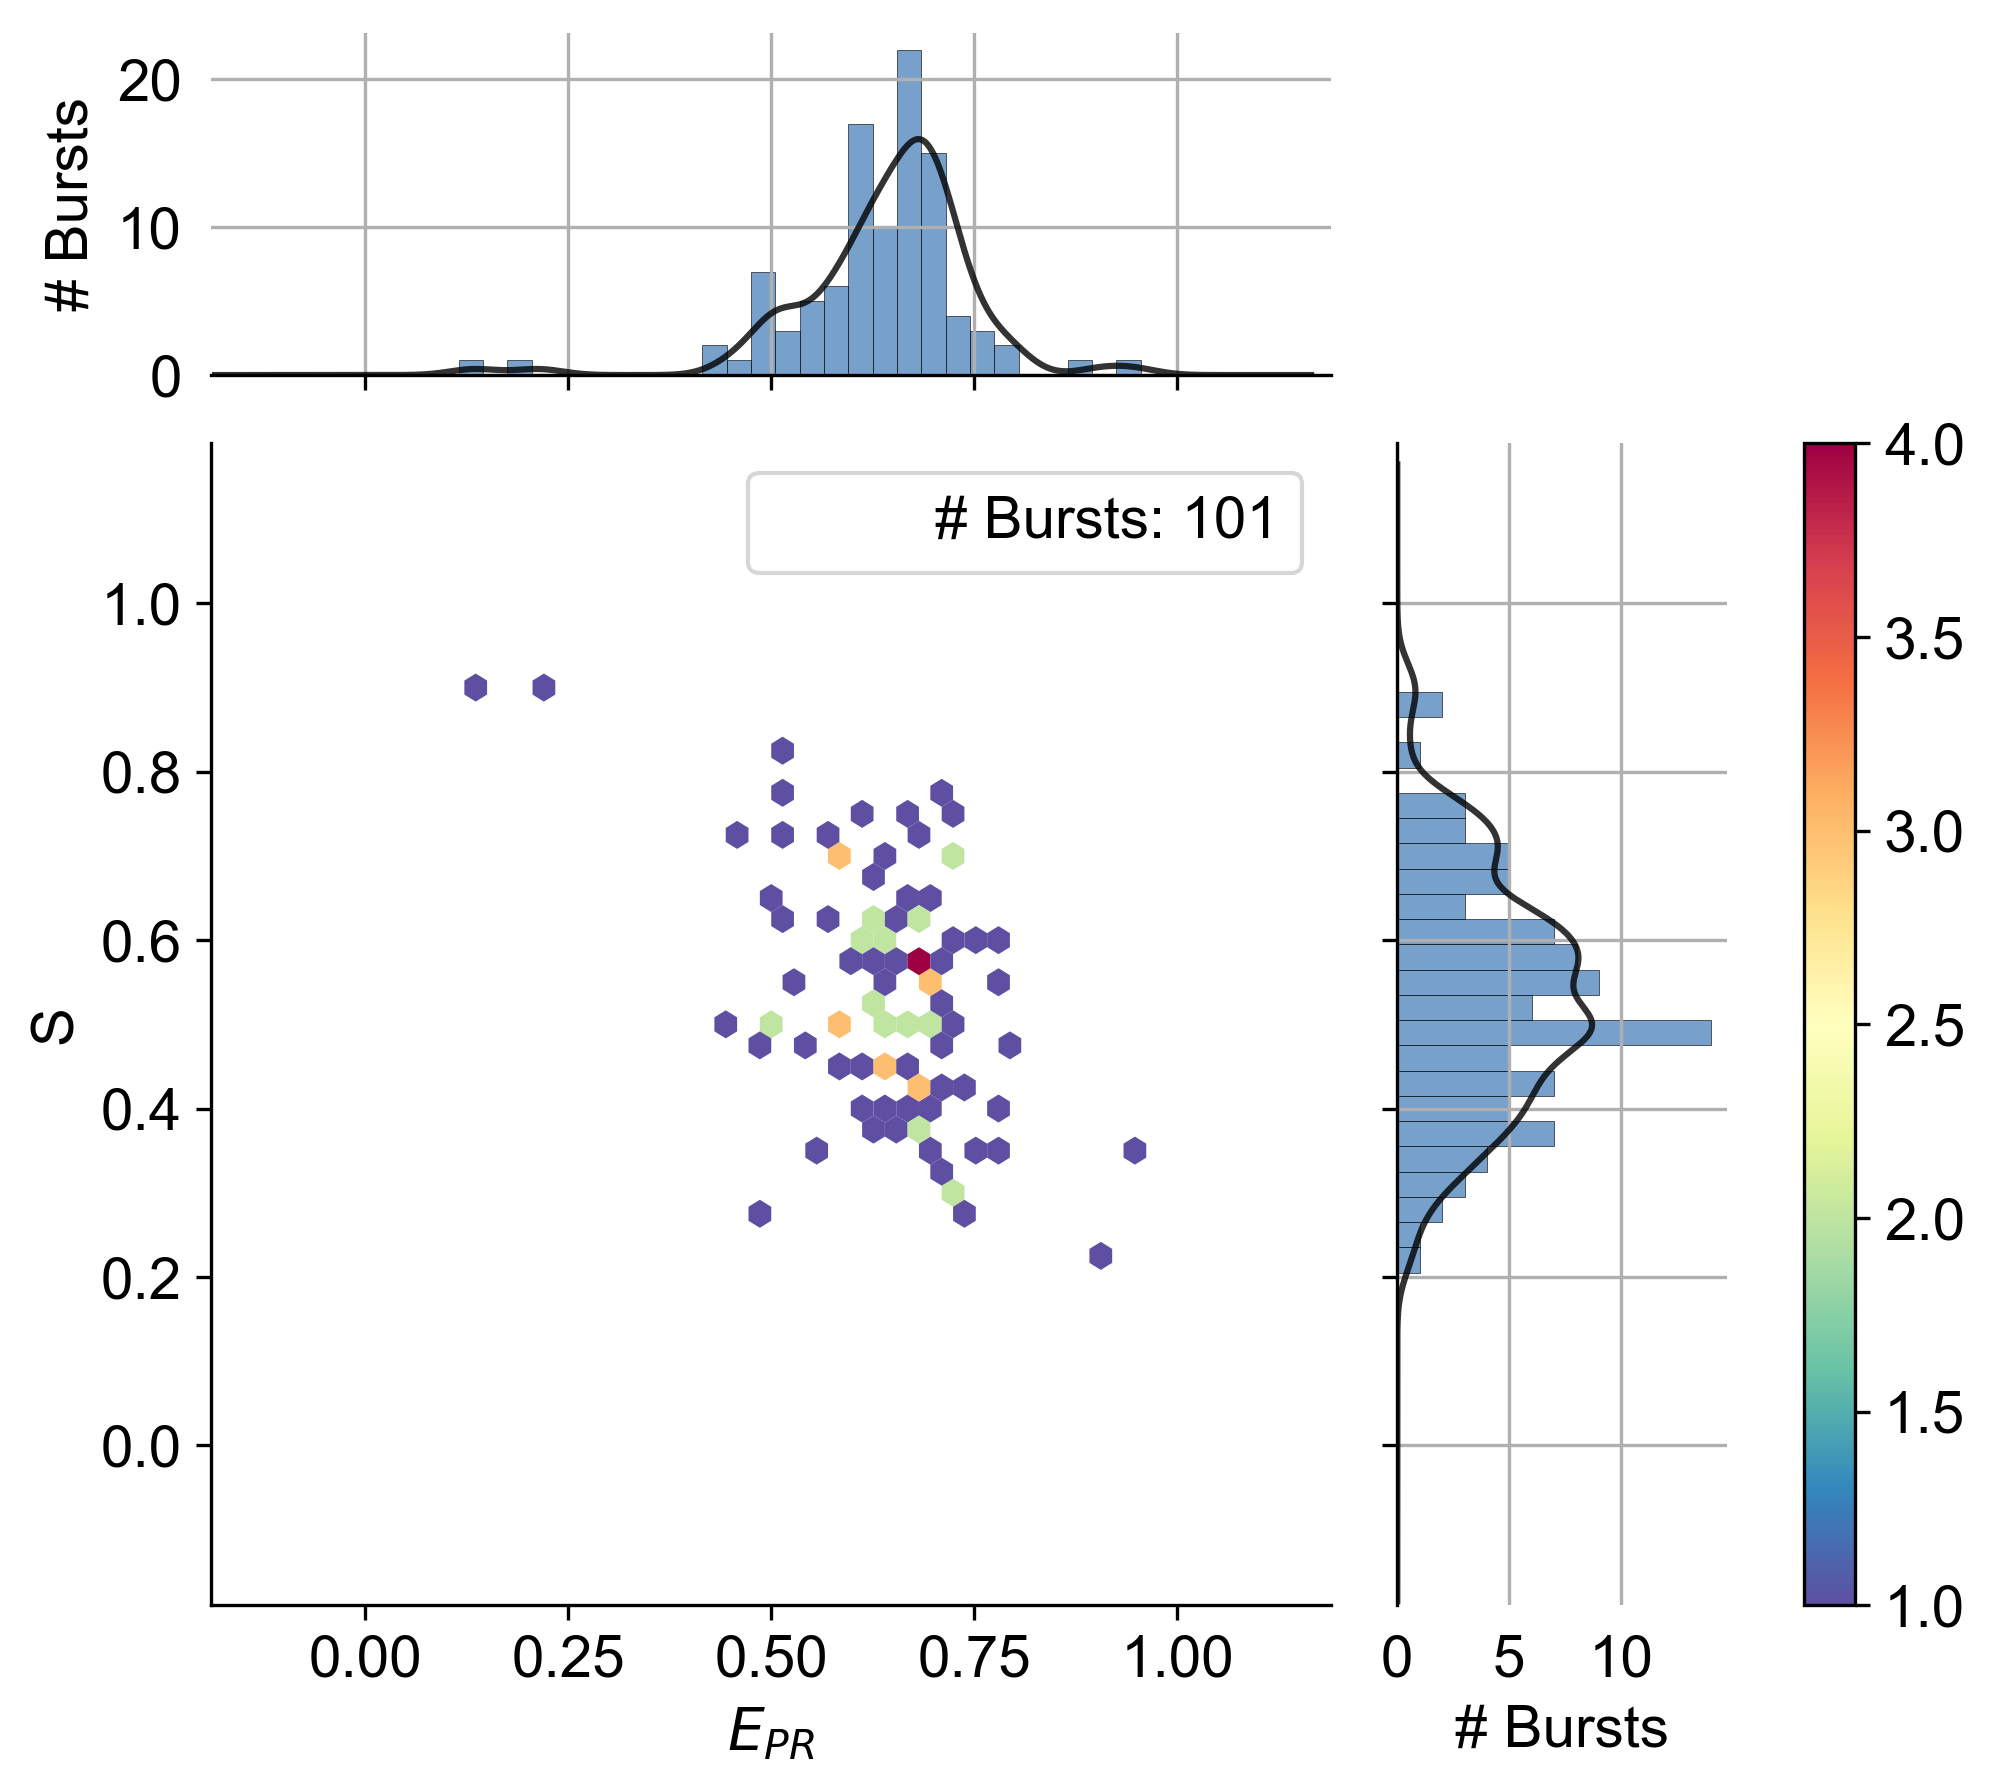
\includegraphics[width=\columnwidth]{figures/2017-06-11_000_12d_alex_jointplot_15s}
\caption{\label{fig:alex_sspot_15}
Single-spot ALEX histogram obtained from 15~s of acquisition for the same
sample as in Fig.~\ref{fig:alex_mspot_15}.}
\end{figure}

\section{Conclusions}

In summary, we have described a new 48-spot single-molecule FRET setup
designed for high-throughput single-molecule assays.
Compared to our previous multispot setup, the number of spots was increased six-fold with a corresponding increase in throughput. While larger SPAD arrays have been fabricated and demonstrated [refs Zappa, Charbon, Henderson], they are fabricated using standard high-voltage CMOS processes not designed for photon detector optimization but instead dense integrated circuit design, resulting in poorer photon-counting performance than the custom technology process employed here. Convincing applications in cell FCS and FLIM (among others) have been published with these CMOS SPAD arrays, but they remain a long way from offering the sensitivity needed for single-molecule applications.
% * <michalet@chem.ucla.edu> 2017-06-16T17:40:44.369Z:
%
% > [refs]
% cite our Zappa collaboration papers, reviews, and the Langowski-Charbon papers, Henderson papers,etc
%
% ^ <michalet@chem.ucla.edu> 2017-06-19T18:43:21.736Z.
Compared to our previous works, a second alternating excitation laser was incorporated, and the corresponding alignment hurdles solved, permitting the sorting of single-molecules according to their donor-acceptor stoichiometry. In particular, we have shown that the setup allows identifying singly- and doubly-labeled species over the full range of FRET efficiencies, opening the door to a much wider range of assays than previously possible.

We presented a detailed description of the multispot setup and alignment procedure,
which incorporates a number of technical solutions of potential interest
for other applications. We also illustrated  the smFRET measurement capabilities of the new setup using doubly-labeled dsDNA molecules  as a proof of principle
demonstration of sub-population separations and high-throughput measurements.
Finally, we provided a comparison of its performance with that
of a standard single-spot (confocal) {\usalex} setup.
Applications of this new instrument to the study of the initial
stages of bacterial transcription and high-throughput diagnostics
will be explored in future work.

\begin{acknowledgments}
This work was supported by NIH grants R01 GM095904 \& R01 GM069709 and
NSF grant MCB 1244175.

Conflict of interest statements: S. Weiss discloses intellectual
property used in the research reported here.
The work at UCLA was conducted in Dr. Weiss's Laboratory.
M. Ghioni discloses equity in Micro Photon Devices S.r.l. (MPD).
No resources or personnel from MPD were involved in this work.
\end{acknowledgments}


\appendix
\section{Appendix: Alignment Protocol}
\label{appendix-alignment-protocol}

\subsection{Signal optimization for coarse alignment of LCOS to SPAD}

Signal is maximized by matching the center of the excitation pattern to
the center of the SPAD array. Figure XXX shows pixel map geometry for
both 12x4 SPAD arrays. The signal across top and bottom regions of the
detector is monitored in labview and the position of the LCOS excitation
pattern is adjusted with respect to the center position of the detector
to maximize the signal. This step allows coarse alignment of excitation
spots to SPADs by maximizing the LCOS-SPAD overlap.


\subsection{Coalignment of SPAD to LCOS pattern by pattern scanning}
\label{coalignment-of-spads-to-lcos-pattern-by-scanning}

After green and red LCOS center positions are coarsely set during signal
optimization, both D and A detectors must be aligned with respect to the
LCOS excitation patterns. SPAD coalignment is achieved by matching SPAD
centers to LCOS centers with automated picomotor controllers (XXX,
reference picomotor control notebook). To this end, scans of center
pixels are collected and analyzed to determine the magnitude and
direction of movement required for alignment. The degree of overlap
between the excitation pattern and SPAD is quantified by a scanning
procedure where the detector is scanned with a 4x4 excitation pattern.
During a multispot scan, a 4x4 LCOS excitation pattern is used to scan
the center of the 12x4 pixel array by moving synchronously across the
4x4 center region in both X and Y directions (reference Appendix Figure
XXX). Scan results are monitored with the acquisition board and SPAD
counts from scanning with the 4x4 LCOS pattern are collected and plotted
against position (reference Appendix Figure XXX). Data from each spot is
fitted with a Gaussian in labview. The process of moving the detector
and scanning the resulting position is repeated until the center
position of the excitation pattern converges with the center position of
the detector to within 0.01 LCOS units.

In practice, alignment of both SPADs to excitation patterns requires
multiple steps. First the D-SPAD is scanned for precise location of
pixel centers using the reference green LCOS configuration from pattern
alignment. The 4x4 LCOS pattern is excited with the 532~nm laser and
excitation spots are used to scan the X and Y locations of pixels at the
center of the D-SPAD. The D-SPAD is moved in LCOS units to match the
center of the green LCOS. After each movement, scans are performed in
triplicate. This is repeated until convergence.

\subsection{Fine X-Y alignment of SPAD}
\label{fine-x-y-alignment-of-spads}

After alignment of the D-SPAD is fixed as previously described, the
A-SPAD is aligned to the D-SPAD by using the reference position of the
green LCOS under 532~nm illumination and moving the A-SPAD with picomotor
control. This step is repeated until center positions of the green LCOS
and A-SPAD converge. Once the centers are matched, the position of the
A-SPAD is fixed. The fixed center position of the A-SPAD is tested with
the red LCOS under 628~nm excitation, and the center location of the red
LCOS is adjusted to maximize overlap of both detectors. It is important
to note that due to spatial constraints the center position of the
A-SPAD can not be adjusted after it is aligned with respect to the green
LCOS, thus a mean position for the center of the red LCOS is selected
based on data from scan fits.


\subsection{Determination of LCOS X-Y pitch and rotation}
\label{x-y-pitch-and-rotation-of-green-and-red-lcoss-by-scan-fits}

Spot rotation and pitch must also be aligned for maximum overlap of
green and red excitation patterns. Alignment of rotation and pitch is an
iterative process that is achieved by calibration of rotation and pitch.
Calibration analysis with Alignment Summary (reference notebook and
supplementary figure showing rotation) is used to extract G and R LCOS
pitch and rotation parameters. Once parameters are determined more scan
are collected to test the quality of overlap between excitation
patterns.

After pitch and rotation of both excitation patterns converge, a final
fine alignment is achieved by matching the center position of the D-SPAD
the center of the green LCOS reference.

\section{Appendix: ALEX and PAX}
\label{sec:alex_pax}

In ALEX, two alternation periods $D_{ex}$ and
$A_{ex}$ (respectively D or A excitation) and two
detectors (D and A) are involved. This results in four basic photon streams named
$D_{ex}D_{em}$, $D_{ex}A_{em}$, $A_{ex}D_{em}$, $A_{ex}A_{em}$, where the first symbol indicate the excitation period and the second, the detection channel.
The $A_{ex}D_{em}$ stream only contains
background because there is no fluorescent emission in the D spectral
band during A-laser excitation. For simplicity, we assume here  that these
quantities are first corrected for
background~\cite{ingargiola_fretbursts:_2016}.

A PAX setup has two detectors (D and A) but only one alternating laser (A).
We can still define two periods, one when only the D laser is on ($D_{ex}$)
and one when both lasers are on (${DA}_{ex}$).
As in ALEX, combining the two
excitation periods and the two detectors leads to four basic PAX
photon streams: $D_{ex}D_{em}$, $D_{ex}A_{em}$, $DA_{ex}D_{em}$, $DA_{ex}A_{em}$.
Formally, the only difference
with the ALEX photon stream is that $A_{ex}$ in ALEX is
replaced with $DA_{ex}$ in PAX. Differently from ALEX, however,
all four photon streams in PAX contain useful fluorescent signal. In
particular, $DA_{ex}D_{em}$ contains D fluorescence due to D laser
excitation, while the corresponding term $A_{ex}D_{em}$ in ALEX
contains only background. With this notation, in both
ALEX and PAX, we can define the total fluorescence signal during D excitation
(e.g.~burst size):

\begin{equation}
    \Lambda = {F_{D_{ex}D_{em}} + F_{FRET}}
    \label{eq:burstsize_raw}
\end{equation}

\noindent where the $F$ quantities are background-corrected photon counts.
$F_{FRET}$ is the A fluorescence due to FRET, computed by
subtracting D-leakage and A-direct-excitation from $F_{D_{ex}A_{em}}$:

\begin{equation}
    F_{FRET} = F_{D_{ex}A_{em}} - Lk\,F_{D_{ex}D_{em}} - Dir
    \label{eq:F_FRET}
\end{equation}

We also need the usual correction factors $\gamma$ and
$\beta$~\cite{lee_accurate_2005}:

\begin{align}
    \gamma &= \frac{\phi_A \, \eta_{A_{det}}^{A_{em}}}
                   {\phi_D \, \eta_{D_{det}}^{D_{em}}} \label{eq:gamma} \\
    \beta &= \frac{I_{A_{ex}}\sigma_{A_{ex}}^A}{I_{D_{ex}}\sigma_{D_{ex}}^D}
    \label{eq:beta}
\end{align}

\noindent where $\phi_A$, $\phi_D$ are the dye quantum yields
and $\eta_{A_{det}}^{A_{em}}$, $\eta_{D_{det}}^{D_{em}}$ are the PDEs of the

D and A channels.
In eq.~\ref{eq:beta}, $I_{A_{ex}}$ and $I_{D_{ex}}$ are A and D excitation
intensities, while $\sigma_{A_{ex}}^A$ and $\sigma_{D_{ex}}^D$
are the dye absorption cross-sections at the respective laser wavelength.
$\beta$ accounts for the difference of D and A dye fluorescence when
each dye is excited by its respective laser.

We can define the $\gamma$-corrected total signal
as~\cite{lee_accurate_2005,ingargiola_applying_2017}:

\begin{equation}
    \Lambda_\gamma = {\gamma\,F_{D_{ex}D_{em}} + F_{FRET}}
    \label{eq:burstsize}
\end{equation}

Differently from $\Lambda$, the quantity $\Lambda_\gamma$ does not change with
FRET (as long as the dyes quantum efficiency does not changes).

With these definitions, we can write the expression for proximity ratio
$E_{PR}$ and FRET efficiency $E$ which are valid for both ALEX and PAX:

\begin{align}
    E_{PR} &= \frac{F_{FRET}}{\Lambda} \label{eq:Epr} \\
    E &= \frac{F_{FRET}}{\Lambda_\gamma} \label{eq:E}
\end{align}

Conversely, the $S$ expression is slightly different for ALEX and PAX. In
ALEX we define $S$ and the corrected version $S_{\gamma\beta}$ as:

\begin{align}
    S &= \frac{\Lambda}{\Lambda + F_{AexAem}} \label{eq:S} \\
    S_{\gamma\beta} &= \frac{\Lambda_\gamma}
                            {\Lambda_\gamma + \frac{F_{AexAem}}{\beta}}
                            \label{eq:Sgb}
\end{align}

The value $S_{\gamma\beta}$ is always centered around 0.5 for dual-labeled
species, regardless of FRET efficiency or D and A excitation intensities.

In PAX, we do not measure the $F_{A_{ex}A_{em}}$ directly, but we can
compute it as:

\begin{equation}
    \tilde{F}_{A_{ex}A_{em}} = F_{DA_{ex}A_{em}} - F_{D_{ex}A_{em}}
    \label{eq:pax_Faa}
\end{equation}

By replacing $F_{A_{ex}A_{em}}$ with $\tilde{F}_{A_{ex}A_{em}}$,
the PAX expressions for $S$ and $S_{\gamma\beta}$ become formally identical
to eq.~\ref{eq:S} and \ref{eq:Sgb}:

\begin{align}
S &= \frac{\Lambda}
          {\Lambda + \tilde{F}_{AexAem}} \label{eq:Spax} \\
S_{\gamma\beta} &= \frac{\Lambda_\gamma}
                        {\Lambda_\gamma + \frac{\tilde{F}_{AexAem}}{\beta}}
         \label{eq:Sgb_pax}
\end{align}

In PAX we can take advantage of the additional signal in
$F_{A_{ex}D_{em}}$ and derive an equivalent set of PAX-enhanced
expressions for $E$ and $S$. We can
start extending the definitions of the total FRET signal of
eq.~\ref{eq:burstsize_raw} and~\ref{eq:burstsize} by including
$F_{A_{ex}D_{em}}$ as follows:

\begin{align}
    \Lambda_{PAX} &= {F_{D_{ex}D_{em}} + F_{A_{ex}D_{em}} + 2 F_{FRET}}
    \label{eq:burstsizerawpaxe} \\
    \Lambda_{\gamma,PAX} &= {\gamma\,(F_{D_{ex}D_{em}} + F_{A_{ex}De_{m}}) + 2 F_{FRET}}
    \label{eq:burstsize_paxe}
\end{align}

Based on eq.~\ref{eq:burstsizerawpaxe} and \ref{eq:burstsize_paxe}, we
can write PAX-enhanced expressions for $E$ and $S$:

\begin{align}
    E_{PR,PAX} &= \frac{2\,F_{FRET}}{\Lambda_{PAX}} \label{eq:Epr_paxe} \\
    E_{PAX} &= \frac{2\,F_{FRET}}{\Lambda_{\gamma,PAX}} \label{eq:Epaxe} \\
    S_{PAX} &= \frac{\Lambda_{PAX}}{\Lambda_{PAX} + \tilde{F}_{A_{ex}A_{em}}}
    \label{eq:Spaxe} \\
    S_{\gamma\beta,PAX} &= \frac{\Lambda_{\gamma,PAX}}
        {\Lambda_{\gamma,PAX} + \frac{2\tilde{F}_{A_{ex}A_{em}}}{\beta}}
    \label{eq:Sgb_paxe}
\end{align}

Eq.~\ref{eq:Epr_paxe}, \ref{eq:Epaxe}, \ref{eq:Spaxe}
and~\ref{eq:Sgb_paxe} contain more photons than the classical expressions
and therefore can result in lower shot-noise. However this effect is
mitigated by the fact that $F_{FRET}$ is counted twice (to
compensate for the doubling of the D signal) and therefore its
shot-noise is amplified.


\subsection{Modified stoichiometry}\label{modified-stoichiometry}

By replacing $\tilde{F}_{A_{ex}A_{em}}$ with $F_{A_{ex}DA_{em}}$ in eq.
\ref{eq:Spax}, we can define a modified stoichiometry $S_u$
as follows

\begin{equation}
S_u = \frac{\Lambda}
{\Lambda + F_{A_{ex}DA_{em}}}
\label{eq:Su}
\end{equation}

This expression avoids the subtraction of photon counts necessary to
compute $\tilde{F}_{A_{ex}A_{em}}$ in PAX (eq.~\ref{eq:pax_Faa}) and the
corresponding increase in shot-noise. As a results, the
$S_u$ distributions are tighter and permit easier
separation of FRET and D-only population, which is the main purpose of
$S$. Note, however, that $S_u$ has a
built-in dependency on the population FRET value, in particular
$S_u$ decreases with the increasing $E$.
Nonetheless, even at low FRET values, better separation between FRET and
D-only population was achieved using $S_u$ instead of
$S$. In principle, once populations are separated, one
can return to use the classical $S$ expression for the
purpose of computing gamma factors. Our interest, in the current paper,
was not recovering absolute FRET values and D-A distances, but rather
demonstrating the capabilities of the smFRET-PAX system in terms of
spot-uniformity and throughput increase. Therefore, we did not compute a
complete gamma factor calibration. However, we addressed the differences
in collection and detection efficiency across the different spots using
a ``relative'' gamma coefficient $\chi_{ch}$ as illustrated in
section \ref{sec:perchcorr}.


\section{Individual channel corrections}

\label{sec:perchcorr}

\subsection{Gamma correction}

The gamma-factor of each channel, $\gamma_{ch}$, can be expressed as the product of
an average factor $\gamma_m$ and a spot-specific adjustment factor
$\chi_{ch}$:

\begin{equation}
\gamma_{ch} = \gamma_m \cdot \chi_{ch}
\label{eq:gamma_split}
\end{equation}

$\chi_{ch}$ can be easily computed from measurable
quantities according to the following expression:

\begin{equation}
\chi_{ch} = \frac{\frac{1}{\langle E_{PR\,ch} \rangle_{ch}} - 1}{\frac{1}{E_{PR\,ch}} - 1}
\label{eq:chich}
\end{equation}

In eq.~\ref{eq:chich}, $E_{PR\,ch}$ is the population-level
proximity ratio for a specific channel, and $ \langle E_{PRch} \rangle_{ch} $ is the
average over all $N$
channels (in this case $N= 48$).

Eq.~\ref{eq:chich} follows from the following relation between $E$
and $E_{PR}$\cite{lee_accurate_2005, ingargiola_applying_2017}:

\begin{equation}
E = f(E_{PR}, \gamma) = \frac{1}{1 + \gamma \left( \frac{1}{E_{PR}} - 1 \right)}
\label{eq:EfuncEpr}
\end{equation}

Solving eq.~\ref{eq:EfuncEpr} for $\gamma$, we obtain:

\begin{equation}
\gamma = \frac{\frac{1}{E} - 1}{\frac{1}{E_{PR}} - 1}
\label{eq:gamma_funcEEpr}
\end{equation}

Formally, we can write $\gamma = \gamma_1 \gamma_2 $, where $\gamma_1$
is associated with a partially corrected
proximity ratio $E_1$ as follows:

\begin{equation}
E_1 = f(E_{PR}, \gamma_1) = \frac{1}{1 + \gamma_1 \left( \frac{1}{E_{PR}} - 1 \right)}
\label{eq:E1funcEpr}
\end{equation}

Writing $\gamma_1$ as a function of $E_1$ as in~\ref{eq:gamma_funcEEpr} and
substituting the expression into eq.~\ref{eq:EfuncEpr},
we obtain $E$ as a function of $E_{1}$:

\begin{equation}
E = f(E_1, \gamma_2) = \frac{1}{1 + \gamma_2 \left( \frac{1}{E_1} - 1 \right)}
\label{eq:EfuncE1}
\end{equation}

Eq.~\ref{eq:EfuncE1} has the same form as \ref{eq:EfuncEpr}
and~\ref{eq:EfuncE1}. Therefore,
$E$ can be obtained by two subsequent (chained) corrections for $\gamma_1$ and
$\gamma_2$ respectively as in eq.~\ref{eq:EfuncEprE1}.

\begin{equation}
E = f(E_{PR}, \gamma) =  f(E_1, \gamma_2) = f(f(E_{PR}, \gamma_1), \gamma_2)
\label{eq:EfuncEprE1}
\end{equation}

In the multispot case, we apply this property to decompose the gamma
correction into a spot-specific correction and an average correction as
in~\ref{eq:gamma_split}.
In particular, eq.~\ref{eq:chich} directly derives from~\ref{eq:gamma_funcEEpr}
with simple substitutions.

\subsection{Beta correction}

Since, formally eq.~\ref{eq:S} and~\ref{eq:Sgb} have the same form as
$E_{PR}$ and $E$, we can write an expression
equivalent to~\ref{eq:EfuncEpr} for $S$ and
$S_{\gamma\beta}$. Dropping the $\gamma$ subscript, we
obtain:

\begin{equation}
S_{\beta} = \frac{1}{1 + \frac{1}{\beta} \left( \frac{1}{S} - 1 \right)}
\label{eq:SbfuncS}
\end{equation}

Following the same arguments as in the previous section,
the beta correction can be expressed as the product of a spot-average $\beta_m$ and an individual channel correction $\beta_{ch}$:

\begin{equation}
\beta = \beta_m \, \beta_{ch}
\label{eq:beta_factor}
\end{equation}

Similarly to eq.~\ref{eq:chich}, we can compute $\beta_{ch}$ as:

\begin{equation}
\frac{1}{\beta_{ch}} = \frac{\frac{1}{\langle S_{ch} \rangle_{ch}} - 1}{\frac{1}{S_{ch}} - 1}
\label{eq:betach}
\end{equation}

\noindent where $S_{ch}$ is the population-level non-beta-corrected
stoichiometry  ratio for a specific channel, and $ \langle S_{ch} \rangle_{ch} $ is the
average over all $N$
channels ($N= 48$ in this case).

\section{Additional data}
% * <michalet@chem.ucla.edu> 2017-06-19T13:33:49.301Z:
%
% > Additional data
% Needs some text?
%
% ^ <michalet@chem.ucla.edu> 2017-06-19T18:51:52.355Z.

\begin{figure*}
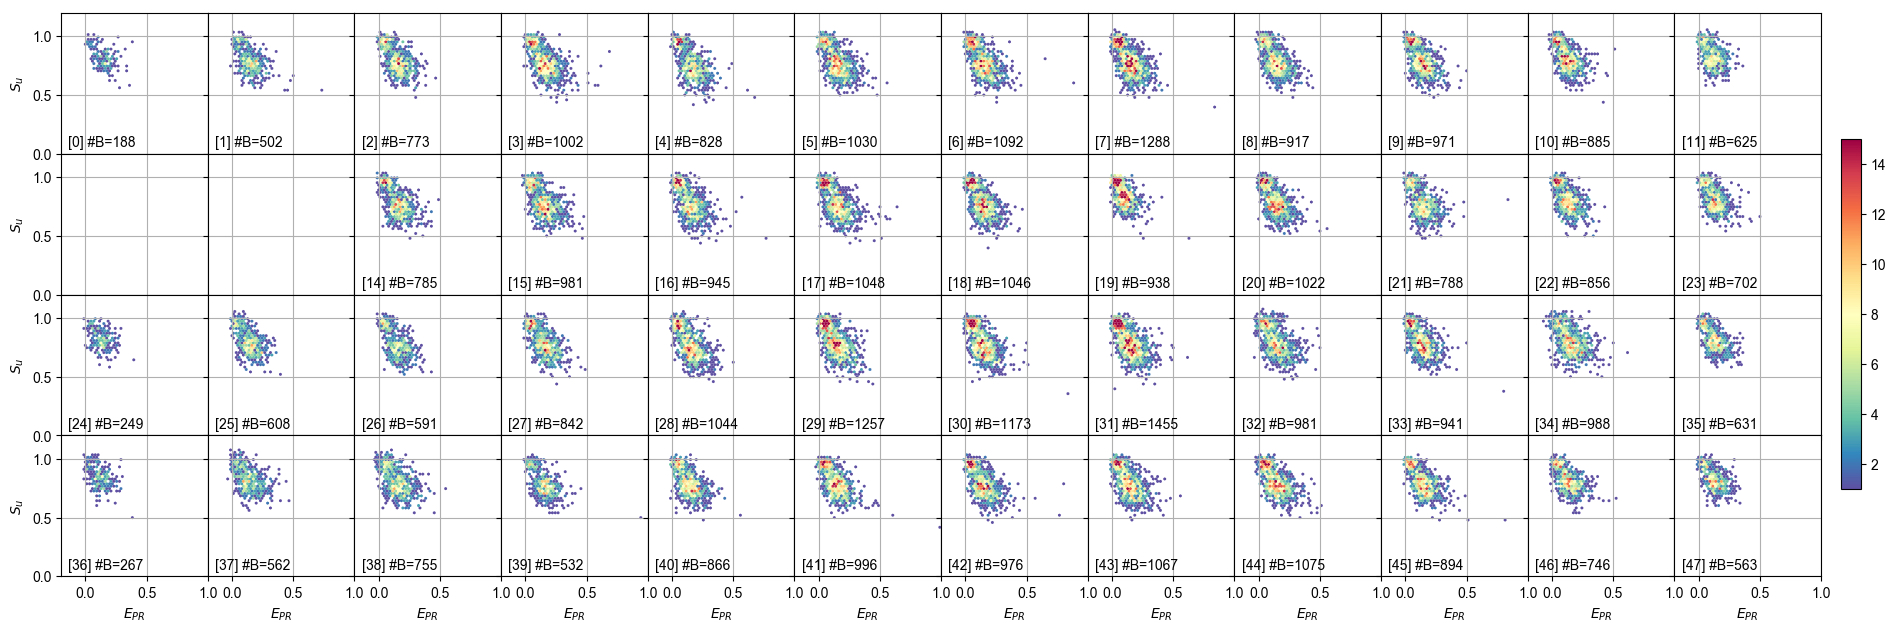
\includegraphics[width=\textwidth]{{figures/2017-05-23_04_22d_48spot_alex_hist_Su_all-bursts}}
\caption{{\label{fig:alexhist48fret2} $E_{PR}$ versus $S_u$
histograms for the different spots for the 22d dsDNA sample. Data and
burst search is identical as in figure~\ref{fig:alexhist48all}, while
burst selection has been tailored to select only the FRET population.
The burst selection criteria is the following: a burst is selected if
counts in $D_{ex}DA_{em}$ stream are larger than 20 and counts in
$DA_{ex}A_{em}$ stream are larger than 20. Text in each subplot
reports spot number ($[\cdot]$) and number of bursts (\#B).%
}}
\end{figure*}

\nocite{*}
\bibliography{biblio}% Produces the bibliography via BibTeX.

\end{document}
%
% ****** End of file aipsamp.tex ******
